\appendix
\part*{附录一：抽象废话}
\addcontentsline{toc}{part}{附录一：抽象废话}
\chapter{富集范畴论基本概念}\label{ch:enriched-category-theory}


\providecommand{\Cat}{\mathcal{C}at}
\providecommand{\sSet}{s\mathcal{S}et}
\providecommand{\Set}{\mathcal{S}et}

\trEnrichedCategory{}论之所以存在，是因为\trEnrichedCategory{}天然存在。为作
说明，试考虑由下列数据给出的一个 1-\trCategory{} $\mathcal{C}$：
\begin{itemize}
\item 对象的一个汇集；
\item 对每一对对象 $x$，$y\in\mathcal{C}$，一个由 $\mathcal{C}$ 中从 $x$ 到%
  $y$ 的箭头组成的集合 $\mathcal{C}(x,y)$；
\item 对每个 $x\in\mathcal{C}$，一个指定的单位元%
  $\mathrm{id}_x\colon 1\to\mathcal{C}(x,x)$；并且对每三个对象 $x$，$y$，%
  $z\in\mathcal{C}$，一个指定的复合映射
  $\circ\colon\mathcal{C}(y,z)\times\mathcal{C}(x,y)\to\mathcal{C}(x,z)$，
  满足下述结合律与单位\footnote{令人困惑的是，这一\trDiagram{}包含两种不同
  样式的恒等箭头：例如，顶部的那条水平箭头便是指定的单位元
  $\mathrm{id}_x\colon 1\to\mathcal{C}(x,x)$ 与相伴于对象 $\mathcal{C}(x,y)$
  的恒等箭头这二者的乘积。}条件：
\end{itemize}

\rvsync{1}%
\begin{rveq}\label{eq:assoc-unit-squares}
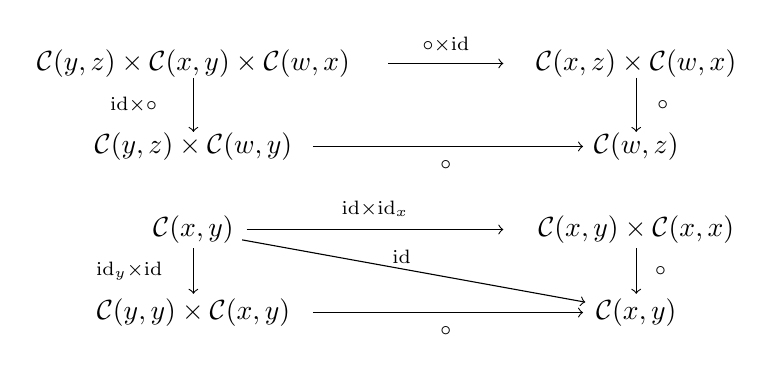
\begin{tikzpicture}[x=1.6em,y=1.5em]
  \node (TL) at (0,2.8)  {$\mathcal{C}(y,z)\times\mathcal{C}(x,y)\times\mathcal{C}(w,x)$};
  \node (TR) at (10,2.8) {$\mathcal{C}(x,z)\times\mathcal{C}(w,x)$};
  \node (BL) at (0,0.8)  {$\mathcal{C}(y,z)\times\mathcal{C}(w,y)$};
  \node (BR) at (10,0.8) {$\mathcal{C}(w,z)$};
  \draw[->] (4.4,2.8) -- (7.0,2.8);
  \node at (5.7,3.25) {$\scriptstyle\circ\times\mathrm{id}$};
  \draw[->] (0,2.45) -- (0,1.15);
  \node at (-1.35,1.8) {$\scriptstyle\mathrm{id}\times\circ$};
  \draw[->] (10,2.45) -- (10,1.15);
  \node at (10.6,1.8) {$\scriptstyle\circ$};
  \draw[->] (2.7,0.8) -- (8.8,0.8);
  \node at (5.7,0.35) {$\scriptstyle\circ$};
  \node (tl2) at (0,-1.2)  {$\mathcal{C}(x,y)$};
  \node (tr2) at (10,-1.2) {$\mathcal{C}(x,y)\times\mathcal{C}(x,x)$};
  \node (bl2) at (0,-3.2)  {$\mathcal{C}(y,y)\times\mathcal{C}(x,y)$};
  \node (br2) at (10,-3.2) {$\mathcal{C}(x,y)$};
  \draw[->] (1.2,-1.2) -- (7.0,-1.2);
  \node at (4.1,-0.7) {$\scriptstyle\mathrm{id}\times\mathrm{id}_x$};
  \draw[->] (0,-1.65) -- (0,-2.75);
  \node at (-1.45,-2.2) {$\scriptstyle\mathrm{id}_y\times\mathrm{id}$};
  \draw[->] (10,-1.65) -- (10,-2.75);
  \node at (10.55,-2.2) {$\scriptstyle\circ$};
  \draw[->] (1.1,-1.45) -- (8.85,-2.95);
  \node at (4.7,-1.85) {$\scriptstyle\mathrm{id}$};
  \draw[->] (2.7,-3.2) -- (8.8,-3.2);
  \node at (5.7,-3.65) {$\scriptstyle\circ$};
\end{tikzpicture}
\end{rveq}

在许多令人感兴趣的数学例子中，集合 $\mathcal{C}(x,y)$ 都可以被赋予额外的
结构；在此情形下，若在施行进一步的范畴论构造时不将它考虑在内，就未免奇怪了。

或许在每个 hom-集中都存在一个指定的零箭头 $0_{x,y}\in\mathcal{C}(x,y)$，它为
复合定义一个双侧理想：$g\circ 0\circ f=0$。或者将此延伸，或许每个
$\mathcal{C}(x,y)$ 都是一个\trAbelianGroup{}，且复合为 $\mathbb{Z}$-\trBilinear。
又或者在另一个方向上，或许 $\mathcal{C}$ 中从 $x$ 到 $y$ 的箭头之集构成某个
1-\trCategory{}的对象。在此设定下，我们把 $\mathcal{C}(x,y)$ 的对象视作
$\mathcal{C}$ 中从 $x$ 到 $y$ 的「$1$ 维」态射，而把 $\mathcal{C}(x,y)$ 的
箭头视作 $\mathcal{C}$ 中从 $x$ 到 $y$ 的「$2$ 维」态射；此处，自然会要求复合
映射定义一个\trFunctor。又或许，$\mathcal{C}$ 中从 $x$ 到 $y$ 的箭头之集构成
一个\trSimplicialSet{}的顶点，其更高维的诸\trSimplex{}便在每个正维数下提供
箭头；此处，自然会要求复合定义一个\trSimplicialMap。在上述所有情境中，人们说
1-\trCategory{} $\mathcal{C}$ 可以\emph{在范畴 $\mathcal{V}$ 上富集}——%
$\mathcal{V}$ 即诸对象 $\mathcal{C}(x,y)$ 与诸\trDiagram{}
\eqref{eq:assoc-unit-squares} 所栖居\footnote{要在 $\mathcal{V}$ 中诠释%
\trDiagram{} \eqref{eq:assoc-unit-squares}，需要为\trMonoidalProduct「$\times$」及其
单位对象 $1$ 指定一种诠释（图中并未将后者显示出来）。在我们考虑的诸例中，
这一乘积是笛卡尔积，而这一单位是\trTerminal{}对象。}的那个范畴；在刚才描述
的诸例中，$\mathcal{V}$ 分别为带点的集合的范畴、\trAbelianGroup{}的范畴、%
\trCategory{}的范畴，或\trSimplicialSet{}的范畴。
关于\trEnrichedCategory{}论的另一种观点也常被强调——例如经典教科书%
\cite{bib68} 便采纳了这一观点，而本章的标题正是从它那里偷来的。借用%
Peter May 使用过的一个区分，术语「富集」既可以用作复合名词——%
\emph{\trEnrichedCategory}——也可以用作形容词——\emph{富集的}\trCategory。
在名词形态下，\trEnrichedCategory{} $\mathcal{C}$ 并没有先在的底通常范畴，
不过我们将会在\cref{def:underlying-category}中看到：底下的非富集 1-\trCategory{}总能够被事后
辨认出来。
而当用作形容词时，一个\trEnrichedCategory{} $\mathcal{C}$ 或许最自然地就是
一个通常范畴，其诸 hom-集可以被赋予额外的结构。\footnote{试引 \cite{bib84}
的话：「同时从这两个观点出发进行思考，至关重要的一点在于：所构造出的通常
范畴与人们最初着手的那一通常范畴是同构的。不论采取哪种观点，范畴论家所
偏好的记号与『从事实际工作的数学家』所通用的记号之间都存在冲突
（\cite{bib81} 所面向的读者正是后者）。」}虽然在讨论\trEnrichedCategory{}的
一般理论时，名词视角可以说更为优雅，但在讨论例子时占据主导的却是形容词
视角，因此我们在此选择强调形容词形态，专注于将非富集的范畴加以富集。

在 A.2 节中给出\trEnrichedCategory{}及两者之间富集\trFunctor{}的精确定义
之前，我们在 A.1 节中研究定义富集之基的范畴 $\mathcal{V}$——诸 hom-对象
最终即栖居于其中。本书中出现的首要例子是 $\mathcal{V}=\Cat$ 与
$\mathcal{V}=\sSet$——以及非富集的情形 $\mathcal{V}=\Set$——它们每一个都
具有作为\trCartesianClosed{}范畴的这一特殊性质。既然在\trCartesianClosed{}%
范畴上作富集有若干简化之处，我们便容许自己奢侈一回，显式地以这些基展开
工作。\footnote{更一般地，一个范畴可以在一个\trMonoidalCategory{}
\cite{bib68}、一个\trBicategory（bicategory）\cite{bib17} 或一个%
\trVirtualDoubleCategory{} \cite{bib75} 上富集，其中每一者都推广了前面的诸
富集基。}
我们接着在 A.3 节中介绍富集\trNaturalTransformation{}与富集\trYonedaLemma。
这些概念使我们得以正确地陈述那些在 A.4 节中刻画\emph{\trCotensor}与%
\emph{\trTensor}、在 A.5 节中刻画\emph{锥形极限}与\emph{\trColimit}的%
\trUniversalProperty{}——它们涉及一个富集自然同构。它们各自都是%
\emph{\trWeightedLimit}与\emph{\trWeightedColimit}的特殊情形，后者将在
A.6 节中引入。我们最后在 A.7 节中以「\trChangeOfBase」的一般理论作结——
这是\trEnrichedCategory{}理论中唯一未被 \cite{bib68} 以百科全书式的细节加以
覆盖的部分，其原始文献反而是 \cite{bib41}——它使我们能够更精确地把握下述
过程：一个 2-\trCategory{}如何可以被看作一个\trSimplicialCategory，或者一个%
\trSimplicialCategory{}如何可以经作商而定义一个 2-\trCategory，一如第 1 章
中的\cref{dig:change-of-base}所顺带提及的那样。


\providecommand{\Cat}{\mathcal{C}at}
\providecommand{\sSet}{s\mathcal{S}et}

\section{\trCartesianClosed{}\trCategory}\label{sec:cartesian-closed-categories}

在本书通篇中，富集的基\trCategory{}总取为一个\trComplete{}且\trCocomplete{}的%
\trCartesianClosed{}\trCategory：

\begin{definition}\label{def:cartesian-closed}
一个\trCategory{} $\mathcal{V}$ 是\trCartesianClosed，若它
\begin{itemize}
\item 容许有限\trProduct，或者等价地，容许一个\trTerminal{}对象
  $1\in\mathcal{V}$ 与二元\trProduct，并且
\item 对每个 $v\in\mathcal{V}$，\trFunctor{}
  $v\times-\colon\mathcal{V}\to\mathcal{V}$ 容有一个\trRightAdjoint{}
  $(-)^{v}\colon\mathcal{V}\to\mathcal{V}$。
\end{itemize}
\end{definition}

\begin{lemma}\label{lem:two-variable-adjunction}
在一个\trCartesianClosed{}\trCategory{} $\mathcal{V}$ 中，乘积\trBifunctor{}是
一个双变量\trAdjunction{}的\trLeftAdjoint，这由一个由自然\trIsomorphism{}组成
的交换三角形所刻画：
\begin{rveq}\label{eq:two-variable-adjunction-isos}
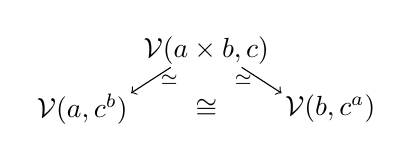
\begin{tikzpicture}[x=1.6em,y=1.5em]
  \node (t)  at (2.8,1.4) {$\mathcal{V}(a\times b,c)$};
  \node (bl) at (0,0)   {$\mathcal{V}(a,c^{b})$};
  \node (br) at (5.6,0) {$\mathcal{V}(b,c^{a})$};
  \draw[->] (2.0,1.0) -- node[right]{$\scriptstyle\simeq$} (1.1,0.38);
  \draw[->] (3.6,1.0) -- node[left]{$\scriptstyle\simeq$} (4.5,0.38);
  \node at (2.8,0) {$\cong$};
\end{tikzpicture}
\end{rveq}
\end{lemma}

\begin{proof}
诸\trFunctor{} $(-)^{a}\colon\mathcal{V}\to\mathcal{V}$ 之族以一种唯一的方式
扩张为\trBifunctor
\[ (-)^{-}\colon\mathcal{V}^{\mathrm{op}}\times\mathcal{V}\to\mathcal{V} \]
使得定义每个\trAdjunction{} $a\times-\dashv(-)^{a}$ 的那些同构
\[ \mathcal{V}(a\times b,c)\cong\mathcal{V}(b,c^{a}) \]
在 $a$ 上（同样也在 $b$ 与 $c$ 上）成为自然的。细节留作%
\cref{ex:extend-to-bifunctors}（或见 \cite[4.3.6]{bib104}）。这就定义了
\eqref{eq:two-variable-adjunction-isos} 右侧的那个自然\trIsomorphism。左侧的
自然\trIsomorphism{}则由与对称\trIsomorphism{} $a\times b\cong b\times a$ 作
复合而定义。第三个自然\trIsomorphism{}取为这两者的复合。
\end{proof}

\begin{example}[\trCartesianClosed{}\trCategory]\label{exa:cartesian-closed-examples}
\begin{enumerate}[label=(\roman*)]
\item 集合的\trCategory{}是\trCartesianClosed，其中 $B^{A}$ 定义为从 $A$
  到 $B$ 的函数之集。跨越自然\trIsomorphism{}
  \eqref{eq:two-variable-adjunction-isos} 的转置被称为「柯里化」（currying）。
\item 小\footnote{一般地，其态射之集被某个固定的不可达基数所界定的诸%
\trCategory{}所组成的\trCategory，在该 Grothendieck 宇宙中是%
\trCartesianClosed{}。}\trCategory{}的\trCategory{} $\Cat$ 是%
\trCartesianClosed{}，其中 $B^{A}$ 定义为从 $A$ 到 $B$ 的诸\trFunctor{}与诸%
\trNaturalTransformation{}的\trCategory。
\[ \Cat(A,C^{B})\cong\Cat(A\times B,C)\cong\Cat(B,C^{A}) \]
上式把诸\trNaturalTransformation{}——即函子\trCategory{}中的箭头
$2\to C^{A}$——与「有向同伦」$A\times 2\to C$ 等同起来。
\item 对任何小\trCategory{} $\mathcal{C}$，\trCategory{}
  $\mathcal{S}et^{\mathcal{C}^{\mathrm{op}}}$ 是\trCartesianClosed。由%
\trYonedaLemma，对 $F,G\in\mathcal{S}et^{\mathcal{C}^{\mathrm{op}}}$，$G^{F}$
在 $c\in\mathcal{C}$ 处的取值必须经由
\[ G^{F}(c)\cong\mathcal{S}et^{\mathcal{C}^{\mathrm{op}}}(\mathcal{C}(-,c),G^{F})
   \cong\mathcal{S}et^{\mathcal{C}^{\mathrm{op}}}(F\times\mathcal{C}(-,c),G) \]
定义为诸\trNaturalTransformation{} $F\times\mathcal{C}(-,c)\Rightarrow G$ 之
集。依照\cref{lem:two-variable-adjunction}，$G^{F}$ 在一个态射
$f\colon c\to c'\in\mathcal{C}$ 上的作用由与相应的\trNaturalTransformation{}
$f\circ-\colon\mathcal{C}(-,c)\Rightarrow\mathcal{C}(-,c')$ 作\trPreComposition{}来定义。
这就定义了\trFunctor{} $G^{F}$。由于任何\trFunctor{}
$H\in\mathcal{S}et^{\mathcal{C}^{\mathrm{op}}}$ 都典范地是诸可表示对象的一个%
\trColimit，这一定义扩充为所需的自然\trIsomorphism{}
$\mathcal{S}et^{\mathcal{C}^{\mathrm{op}}}(H,G^{F})\cong\mathcal{S}et^{\mathcal{C}^{\mathrm{op}}}(F\times H,G)$。
\item 特别地，取 $\mathcal{C}=\boldsymbol{\Delta}$，单纯集的\trCategory{}
  $\sSet:=\mathcal{S}et^{\boldsymbol{\Delta}^{\mathrm{op}}}$ 是%
\trCartesianClosed{}。
\end{enumerate}
\end{example}

指数 $b^{a}$ 常被称为一个\emph{\trInternalHom}（internal hom）。正如这个名称
所暗示的，\trInternalHom{} $b^{a}$ 可以视为 hom-集 $\mathcal{V}(a,b)$ 沿一个
我们即将引入的\trFunctor{}的\trLifting。

\begin{definition}\label{def:underlying-set-functor}
对任何\trCartesianClosed{}\trCategory{} $\mathcal{V}$，\textbf{底集函子}
（underlying set functor）是\trFunctor
\[ \mathcal{V}\xrightarrow{\ (-)_{0}\coloneqq\mathcal{V}(1,-)\ }\mathcal{S}et \]
它由\trTerminal{}对象 $1\in\mathcal{V}$ 所表示。
\end{definition}

\begin{lemma}\label{lem:underlying-set-of-internal-hom}
在一个\trCartesianClosed{}\trCategory{}中，对任何一对对象
$a,b\in\mathcal{V}$，\trInternalHom{} $b^{a}$ 的底集是 $\mathcal{V}(a,b)$，
亦即：
\[ (b^{a})_{0}\cong\mathcal{V}(a,b). \]
\end{lemma}

\begin{proof}
将\cref{def:underlying-set-functor}与
\eqref{eq:two-variable-adjunction-isos} 相结合：
\[ (b^{a})_{0}:=\mathcal{V}(1,b^{a})\cong\mathcal{V}(1\times a,b)
   \cong\mathcal{V}(a,b) \]
这是因为存在自然\trIsomorphism{} $1\times a\cong a$。
\end{proof}

自然会问：底集之间的一个\trIsomorphism{}能否被「富集」而居于 $\mathcal{V}$
之中——亦即，沿底集函子 $(-)_{0}\colon\mathcal{V}\to\mathcal{S}et$ 而被提升？

\begin{lemma}\label{lem:isos-lift-to-V}
一个\trCartesianClosed{}\trCategory{}的定义性双变量\trAdjunction{}所刻画的诸
自然\trIsomorphism{} \eqref{eq:two-variable-adjunction-isos} 提升至
$\mathcal{V}$：对任何 $a,b,c\in\mathcal{V}$，
\begin{rveq}\label{eq:associativity-triangle-isos}
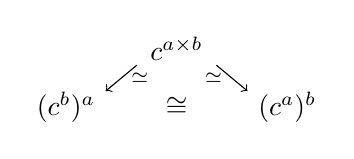
\begin{tikzpicture}[x=1.6em,y=1.5em]
  \node (t)  at (2.5,1.4) {$c^{a\times b}$};
  \node (bl) at (0,0)   {$(c^{b})^{a}$};
  \node (br) at (5.0,0) {$(c^{a})^{b}$};
  \draw[->] (1.6,1.0) -- node[right]{$\scriptstyle\simeq$} (0.9,0.38);
  \draw[->] (3.4,1.0) -- node[left]{$\scriptstyle\simeq$} (4.1,0.38);
  \node at (2.5,0) {$\cong$};
\end{tikzpicture}
\end{rveq}
\end{lemma}

\begin{proof}
这由\cref{lem:two-variable-adjunction}、有限\trProduct{}的结合律以及%
\trYonedaLemma{}推得。为证 \eqref{eq:associativity-triangle-isos}，只需证明
$c^{a\times b}$、$(c^{b})^{a}$ 与 $(c^{a})^{b}$ 表示同一个\trFunctor。通过复合
自然\trIsomorphism{}序列
\begin{align*}
\mathcal{V}(x,(c^{b})^{a})
  &\cong\mathcal{V}(x\times a,c^{b})
    \cong\mathcal{V}((x\times a)\times b,c)
    \cong\mathcal{V}(x\times(a\times b),c)\\
  &\cong\mathcal{V}(x,c^{a\times b})\\
  &\cong\mathcal{V}((a\times b)\times x,c)
    \cong\mathcal{V}(a\times(b\times x),c)
    \cong\mathcal{V}(b\times x,c^{a})\\
  &\cong\mathcal{V}(x,(c^{a})^{b}),
\end{align*}
我们看到
\[ \mathcal{V}(x,(c^{b})^{a})\cong\mathcal{V}(x,c^{a\times b})
   \cong\mathcal{V}(x,(c^{a})^{b}). \]
\end{proof}

\begin{remark}\label{rem:exponent-one-identity}
注意 $(-)^{1}\colon\mathcal{V}\to\mathcal{V}$ 自然\trIsomorphism{}于恒等%
\trFunctor{}——即 $b^{1}\cong b$——因为它是\trFunctor{}
$-\times1\colon\mathcal{V}\to\mathcal{V}$ 的\trRightAdjoint，而后一\trFunctor{}%
自然\trIsomorphism{}于恒等。
\end{remark}

一个\trComplete{}且\trCocomplete{}的\trCartesianClosed{}\trCategory{}是%
\trComplete{}且\trCocomplete{}的封闭对称\trMonoidalCategory{}的一个特例——后者
被 Jean Bénabou 称为一个\textbf{宇宙}（cosmos），以表明这样的基是%
\trEnrichedCategory{}理论的理想环境。出于显然的理由，我们在这里将不使用这个
术语，而是代之以「\trComplete{}且\trCocomplete{}的\trCartesianClosed{}\trCategory」
的说法，以凸显\cref{exa:cartesian-closed-examples}中出现的那些\trCategory{}的
某些共同特征。\footnote{Street \cite{bib117} 曾提出一个与之相竞争的、2-范畴论
意义下的\trFibered{}「宇宙」概念，它与我们所考虑的这个概念更为相近；第 1 章
中的\cref{def:infinity-cosmos}所引入的术语正是直接受其启发。}

\subsection*{练习}

\begin{exercise}\label{ex:extend-to-bifunctors}
证明：在一个\trCartesianClosed{}\trCategory{} $\mathcal{V}$ 中，诸\trFunctor{}
$(-)^{a}\colon\mathcal{V}\to\mathcal{V}$ 之族以一种唯一的方式扩张为\trBifunctor
\[ (-)^{-}\colon\mathcal{V}^{\mathrm{op}}\times\mathcal{V}\to\mathcal{V} \]
使得定义每个\trAdjunction{} $a\times-\dashv(-)^{a}$ 的那个同构
\[ \mathcal{V}(a\times b,c)\cong\mathcal{V}(b,c^{a}) \]
在 $a$ 上（同样也在 $b$ 与 $c$ 上）成为自然的。
\end{exercise}

\begin{exercise}\label{ex:closed-symmetric-monoidal}
一个\textbf{封闭对称幺半范畴}（closed symmetric monoidal category）的数据经由
下述方式推广\cref{def:cartesian-closed}：把有限\trProduct{}换成一个任意的%
\trBifunctor{} $-\otimes-\colon\mathcal{V}\times\mathcal{V}\to\mathcal{V}$，把%
\trTerminal{}对象换成一个对象 $I\in\mathcal{V}$，并额外要求指定诸自然%
\trIsomorphism
\[
a\otimes(b\otimes c)\mathrel{\underset{\alpha}{\cong}}(a\otimes b)\otimes c
\qquad
I\otimes a\mathrel{\underset{\lambda}{\cong}}a
\mathrel{\underset{\rho}{\cong}}a\otimes I
\qquad
a\otimes b\mathrel{\underset{\gamma}{\cong}}b\otimes a
\]
其满足种种相干公理 \cite{bib41,bib66}（另见 \cite{bib69}）。请在%
\trCartesianClosed{}\trCategory{}这一特殊情形下给出这些\trIsomorphism{}的一个%
\trCanonical{}构造，并解释为什么诸相干条件是自动成立的。
\end{exercise}

   %

\providecommand{\Cat}{\mathcal{C}at}
\providecommand{\sSet}{s\mathcal{S}et}

\section{\trEnrichedCategory{}与富集函子}\label{sec:enriched-categories-and-enriched-functors}

现在我们短暂地切换视角，先解释名词短语「\trEnrichedCategory」的含义，然后再
讨论把一个通常的 1-\trCategory{}「富集」起来需要些什么。从本节起直到 A.6 节，
我们固定一个\trComplete{}且\trCocomplete{}的\trCartesianClosed{}\trCategory{}
$(\mathcal{V},\times,1)$ 作为富集所用的基。

\begin{definition}\label{def:enriched-category}
一个 \textbf{$\mathcal{V}$-富集范畴}（$\mathcal{V}$-enriched category）或%
\textbf{$\mathcal{V}$-范畴}（$\mathcal{V}$-category）$\mathcal{C}$ 由如下数据
给出：
\begin{itemize}
\item 对象的一个汇集；%
\item 对每对对象 $x,y\in\mathcal{C}$，一个 \textbf{hom-对象}（hom-object）
  $\mathcal{C}(x,y)\in\mathcal{V}$；
\item 对每个 $x\in\mathcal{C}$，一个指定的 \textbf{单位元}（identity
  element），由映射 $\mathrm{id}_{x}\colon 1\to\mathcal{C}(x,x)\in\mathcal{V}$
  编码；并且对每个 $x,y,z\in\mathcal{C}$，一个指定的 \textbf{复合映射}
  （composition map）
  $\circ\colon\mathcal{C}(y,z)\times\mathcal{C}(x,y)\to\mathcal{C}(x,z)\in\mathcal{V}$，
  其满足结合性与单位这两组条件，两个交换图表均居于
  $\mathcal{V}$ 之中。\footnote{这些图表省去了涉及乘积\trBifunctor{} $\times$
  及其单位对象 $1$ 的那些结合性与单位自然\trIsomorphism。在一个%
  \trCartesianClosed{}\trCategory{}中，这些自然\trIsomorphism{}是
  \emph{典范的}——而非作为额外数据给出；在更一般的\emph{封闭对称幺半范畴}的
  情形中它们则作为额外数据给出（见\cref{ex:closed-symmetric-monoidal}）。}
\end{itemize}
\begin{center}
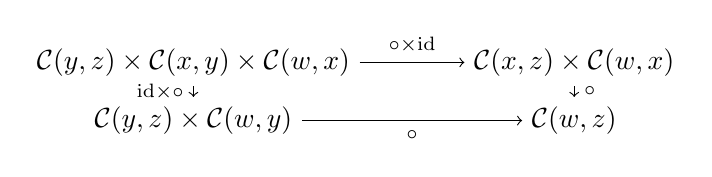
\begin{tikzpicture}[x=1.6em,y=1.5em]
  \node (tl) at (0,1.4)
    {$\mathcal{C}(y,z)\times\mathcal{C}(x,y)\times\mathcal{C}(w,x)$};
  \node (tr) at (8.6,1.4) {$\mathcal{C}(x,z)\times\mathcal{C}(w,x)$};
  \node (bl) at (0,0) {$\mathcal{C}(y,z)\times\mathcal{C}(w,y)$};
  \node (br) at (8.6,0) {$\mathcal{C}(w,z)$};
  \draw[->] (tl) -- node[above]{$\scriptstyle\circ\times\mathrm{id}$} (tr);
  \draw[->] (tl) -- node[left]{$\scriptstyle\mathrm{id}\times\circ$} (bl);
  \draw[->] (tr) -- node[right]{$\scriptstyle\circ$} (br);
  \draw[->] (bl) -- node[below]{$\scriptstyle\circ$} (br);
\end{tikzpicture}

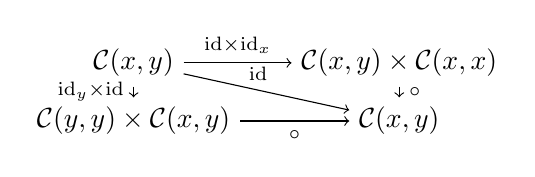
\begin{tikzpicture}[x=1.6em,y=1.5em]
  \node (tl) at (0,1.4) {$\mathcal{C}(x,y)$};
  \node (tr) at (6.0,1.4) {$\mathcal{C}(x,y)\times\mathcal{C}(x,x)$};
  \node (bl) at (0,0) {$\mathcal{C}(y,y)\times\mathcal{C}(x,y)$};
  \node (br) at (6.0,0) {$\mathcal{C}(x,y)$};
  \draw[->] (tl) -- node[above]{$\scriptstyle\mathrm{id}\times\mathrm{id}_{x}$} (tr);
  \draw[->] (tl) -- node[left]{$\scriptstyle\mathrm{id}_{y}\times\mathrm{id}$} (bl);
  \draw[->] (tl) -- node[above,pos=0.45]{$\scriptstyle\mathrm{id}$} (br);
  \draw[->] (tr) -- node[right]{$\scriptstyle\circ$} (br);
  \draw[->] (bl) -- node[below]{$\scriptstyle\circ$} (br);
\end{tikzpicture}
\end{center}
\end{definition}

显然，由\eqref{eq:assoc-unit-squares}的图表可见，一个局部小的 1-\trCategory{}定义了一个富集于
$\mathcal{S}et$ 之上的\trCategory。\cref{def:underlying-set-functor}的底集
函子可用来定义一个富集\trCategory{}的「底范畴」。

\begin{definition}\label{def:underlying-category}
若 $\mathcal{C}$ 是一个 $\mathcal{V}$-范畴，其 \textbf{底范畴}（underlying
category）$\mathcal{C}_{0}$ 是具有相同对象之集的 1-\trCategory，其 hom-集由把
底集函子 $(-)_{0}\colon\mathcal{V}\to\mathcal{S}et$ 施于诸 hom-对象
$\mathcal{C}(x,y)\in\mathcal{V}$ 上而定义。在多数情形下，我们对 hom-对象与
hom-集均写作「$\mathcal{C}(x,y)$」并以措辞来消歧，但必要时
「$\mathcal{C}(x,y)_{0}$」也是底范畴之 hom-集的一种常用记法。
\end{definition}

注意：$\mathcal{V}$-范畴的恒等箭头 $\mathrm{id}_{x}\colon 1\to\mathcal{C}(x,x)$
按定义是 hom-集 $\mathcal{C}(x,x)_{0}:=\mathcal{V}(1,\mathcal{C}(x,x))$ 的一个%
\trElement。底范畴中两支箭头 $f\colon 1\to\mathcal{C}(x,y)$ 与
$g\colon 1\to\mathcal{C}(y,z)$ 的复合，定义为如下复合所构造出的那支箭头
\[ 1\xrightarrow{\ g\times f\ }\mathcal{C}(y,z)\times\mathcal{C}(x,y)
   \xrightarrow{\ \circ\ }\mathcal{C}(x,z) \]

与围绕\cref{def:underlying-set-functor}的讨论相类比，当人们谈及把一个先验非
富集的\trCategory{} $\mathcal{C}$ 「富集」于 $\mathcal{V}$ 之上时，任务便是
定义一个如\cref{def:enriched-category}中的 $\mathcal{V}$-富集范畴，使其底范畴
恢复出 $\mathcal{C}$。当 $\mathcal{V}=\Cat$ 时，任务是定义一个 2-\trCategory，
使其底 1-\trCategory{}即为所给者。当 $\mathcal{V}=\sSet$ 时，任务是定义诸
$n$-箭头的单纯 hom-集，使得 0-箭头即为所给者。当一个%
\trSimpliciallyEnrichedCategory{} $\mathcal{C}$ 如第 1 章中的%
\cref{dig:simplicial-categories}所解释的那样被
编码为 $\Cat$ 中的一个\trSimplicialObject{} $\mathcal{C}_{\bullet}$ 时，其底
范畴便是\trCategory{} $\mathcal{C}_{0}$，这进一步佐证了%
\cref{def:underlying-category}中引入的概念。

例如，\cref{def:cartesian-closed}中那样的一个\trCartesianClosed{}\trCategory{}
$\mathcal{V}$ 可被富集而定义出一个 $\mathcal{V}$-范畴。

\begin{lemma}\label{lem:cartesian-closed-v-category}
一个\trCartesianClosed{}\trCategory{} $\mathcal{V}$ 定义一个 $\mathcal{V}$-范畴，
其：
\begin{itemize}
\item 对象为 $\mathcal{V}$ 的对象；
\item 居于 $\mathcal{V}$ 中、从 $a$ 到 $b$ 的 hom-对象是\trInternalHom{}
  $b^{a}$；
\item 恒等映射 $\mathrm{id}_{a}\colon 1\to a^{a}$ 与复合映射
  $\circ\colon c^{b}\times b^{a}\to c^{a}$ 定义为
  \[ 1\times a\simeq a \qquad\text{以及}\qquad
     c^{b}\times b^{a}\times a
     \xrightarrow{\ \mathrm{id}\times\mathrm{ev}\ }c^{b}\times b
     \xrightarrow{\ \mathrm{ev}\ }c \]
  的转置，后者使用笛卡尔封闭伴随的余单位 $\mathrm{ev}$ 来定义。
\end{itemize}
\end{lemma}

\begin{proof}
任务是验证\cref{def:enriched-category}中的两个交换图表在 $\mathcal{V}$ 中
成立，然后观察到\cref{lem:underlying-set-of-internal-hom}揭示了：由本陈述所
定义的 $\mathcal{V}$-范畴的底范畴正是 1-\trCategory{} $\mathcal{V}$。我们把
恒等条件留给读者，在此验证结合性。

把复合映射定义为伴随转置，这蕴涵它的伴随转置——即下方的右上复合——由左下
复合给出：
\begin{rveq}\label{eq:composition-transpose-square}
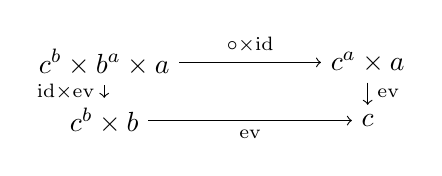
\begin{tikzpicture}[x=1.7em,y=1.5em]
  \node (tl) at (0,1.4) {$c^{b}\times b^{a}\times a$};
  \node (tr) at (5.6,1.4) {$c^{a}\times a$};
  \node (bl) at (0,0) {$c^{b}\times b$};
  \node (br) at (5.6,0) {$c$};
  \draw[->] (tl) -- node[above]{$\scriptstyle\circ\times\mathrm{id}$} (tr);
  \draw[->] (tl) -- node[left]{$\scriptstyle\mathrm{id}\times\mathrm{ev}$} (bl);
  \draw[->] (tr) -- node[right]{$\scriptstyle\mathrm{ev}$} (br);
  \draw[->] (bl) -- node[below]{$\scriptstyle\mathrm{ev}$} (br);
\end{tikzpicture}
\end{rveq}
下左侧的结合性图表交换，当且仅当下右侧作为外边界复合出现的那张转置后的图表
交换：
\begin{center}
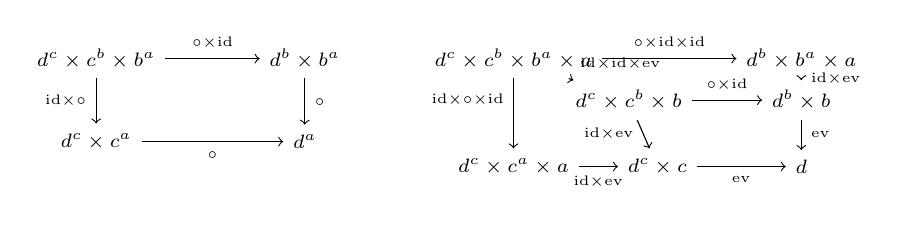
\begin{tikzpicture}[x=1.3em,y=1.5em,every node/.style={font=\scriptsize}]
  \node (LTL) at (0,2.9) {$d^{c}\times c^{b}\times b^{a}$};
  \node (LTR) at (5.8,2.9) {$d^{b}\times b^{a}$};
  \node (LBL) at (0,0.9) {$d^{c}\times c^{a}$};
  \node (LBR) at (5.8,0.9) {$d^{a}$};
  \draw[->] (LTL) -- node[above]{$\scriptstyle\circ\times\mathrm{id}$} (LTR);
  \draw[->] (LTL) -- node[left]{$\scriptstyle\mathrm{id}\times\circ$} (LBL);
  \draw[->] (LTR) -- node[right]{$\scriptstyle\circ$} (LBR);
  \draw[->] (LBL) -- node[below]{$\scriptstyle\circ$} (LBR);
  \node at (7.9,1.9) {$\rightsquigarrow$};
  \node (T)  at (11.6,2.9) {$d^{c}\times c^{b}\times b^{a}\times a$};
  \node (TR) at (19.6,2.9) {$d^{b}\times b^{a}\times a$};
  \node (IL) at (14.8,1.9) {$d^{c}\times c^{b}\times b$};
  \node (IR) at (19.6,1.9) {$d^{b}\times b$};
  \node (BL) at (11.6,0.3) {$d^{c}\times c^{a}\times a$};
  \node (BM) at (15.6,0.3) {$d^{c}\times c$};
  \node (BR) at (19.6,0.3) {$d$};
  \draw[->] (T) -- node[above]{$\scriptstyle\circ\times\mathrm{id}\times\mathrm{id}$} (TR);
  \draw[->] (T) -- node[left,pos=0.3]{$\scriptstyle\mathrm{id}\times\circ\times\mathrm{id}$} (BL);
  \draw[->] (T) -- node[above right,pos=0.35]{$\scriptstyle\mathrm{id}\times\mathrm{id}\times\mathrm{ev}$} (IL);
  \draw[->] (IL) -- node[above]{$\scriptstyle\circ\times\mathrm{id}$} (IR);
  \draw[->] (IL) -- node[left,pos=0.5]{$\scriptstyle\mathrm{id}\times\mathrm{ev}$} (BM);
  \draw[->] (TR) -- node[right]{$\scriptstyle\mathrm{id}\times\mathrm{ev}$} (IR);
  \draw[->] (IR) -- node[right]{$\scriptstyle\mathrm{ev}$} (BR);
  \draw[->] (BL) -- node[below]{$\scriptstyle\mathrm{id}\times\mathrm{ev}$} (BM);
  \draw[->] (BM) -- node[below]{$\scriptstyle\mathrm{ev}$} (BR);
\end{tikzpicture}
\end{center}
这由 $\times$ 的二函子性以及上方交换方块的两个实例推得。
\end{proof}

\begin{definition}\label{def:free-v-category}
1-\trCategory{} $\mathcal{C}$ 上的 \textbf{自由 $\mathcal{V}$-范畴}（free
$\mathcal{V}$-category）具有与之相同的对象之集，其 hom-对象定义为以 hom-集
$\mathcal{C}(x,y)$ 标引的\trTerminal{}对象 $1\in\mathcal{V}$ 的余积
$\coprod_{\mathcal{C}(x,y)}1$。恒等映射
$\mathrm{id}_{x}\colon 1\to\coprod_{\mathcal{C}(x,x)}1$ 由以恒等箭头标引的那个
分量的包含给出，复合映射则通过让复合函数作用于诸标引集来定义：
\[ \coprod_{\mathcal{C}(y,z)}1\times\coprod_{\mathcal{C}(x,y)}1
   \cong\coprod_{\mathcal{C}(y,z)\times\mathcal{C}(x,y)}1
   \xrightarrow{\ \coprod\circ\ }\coprod_{\mathcal{C}(x,z)}1 \]
\end{definition}

例如，自由 $\Cat$-富集范畴是没有非恒等 2-\trCell{}的那些，而自由
$\sSet$-富集范畴则是在正维数中没有非退化箭头的那些。我们对 1-\trCategory{}
$\mathcal{C}$ 与它所生成的自由 $\mathcal{V}$-范畴使用相同的记号，并以措辞来
消歧。

\begin{definition}\label{def:v-enriched-functor}
一个 \textbf{$\mathcal{V}$-富集函子}（$\mathcal{V}$-enriched functor）或
\textbf{$\mathcal{V}$-函子}（$\mathcal{V}$-functor）
$F\colon\mathcal{C}\to\mathcal{D}$ 由如下数据给出：
\begin{itemize}
\item 对象上的一个映射，把每个 $x\in\mathcal{C}$ 送到某个 $Fx\in\mathcal{D}$；
\item 对每对对象 $x,y\in\mathcal{C}$，hom-对象上的一个内部作用，由态射
  $F_{x,y}\colon\mathcal{C}(x,y)\to\mathcal{D}(Fx,Fy)\in\mathcal{V}$ 给出，
  使得 $\mathcal{V}$-函子性图表交换：
\end{itemize}
\begin{center}
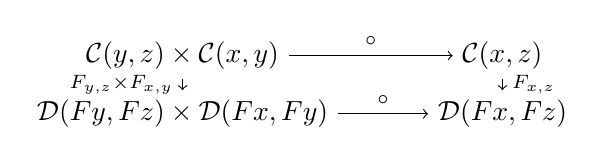
\begin{tikzpicture}[x=1.7em,y=1.5em]
  \node (tl) at (0,1.4) {$\mathcal{C}(y,z)\times\mathcal{C}(x,y)$};
  \node (tr) at (6.8,1.4) {$\mathcal{C}(x,z)$};
  \node (bl) at (0,0) {$\mathcal{D}(Fy,Fz)\times\mathcal{D}(Fx,Fy)$};
  \node (br) at (6.8,0) {$\mathcal{D}(Fx,Fz)$};
  \draw[->] (tl) -- node[above]{$\scriptstyle\circ$} (tr);
  \draw[->] (tl) -- node[left]{$\scriptstyle F_{y,z}\times F_{x,y}$} (bl);
  \draw[->] (tr) -- node[right]{$\scriptstyle F_{x,z}$} (br);
  \draw[->] (bl) -- node[above]{$\scriptstyle\circ$} (br);
\end{tikzpicture}
\qquad
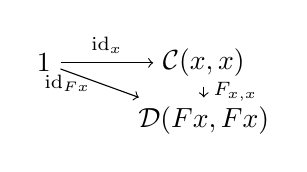
\begin{tikzpicture}[x=1.7em,y=1.5em]
  \node (t)  at (0,1.4) {$1$};
  \node (tr) at (3.4,1.4) {$\mathcal{C}(x,x)$};
  \node (b)  at (3.4,0) {$\mathcal{D}(Fx,Fx)$};
  \draw[->] (t) -- node[above]{$\scriptstyle\mathrm{id}_{x}$} (tr);
  \draw[->] (tr) -- node[right]{$\scriptstyle F_{x,x}$} (b);
  \draw[->] (t) -- node[left]{$\scriptstyle\mathrm{id}_{Fx}$} (b);
\end{tikzpicture}
\end{center}
\end{definition}

一个原型性的例子由可表示函子给出：

\begin{example}\label{exa:enriched-representable}
对任何 $\mathcal{V}$-范畴 $\mathcal{C}$ 与对象 $c\in\mathcal{C}$，\textbf{富集
可表示 $\mathcal{V}$-函子}（enriched representable $\mathcal{V}$-functor）
$\mathcal{C}(c,-)\colon\mathcal{C}\to\mathcal{V}$ 在对象上由指定
$x\in\mathcal{C}\mapsto\mathcal{C}(c,x)\in\mathcal{V}$ 来定义，其在 hom-对象上
的内部作用则定义为 $\mathcal{C}$ 的内部复合映射的伴随转置：
\[ \mathcal{C}(x,y)\xrightarrow{\ \mathcal{C}(c,-)_{x,y}\ }
   \mathcal{C}(c,y)^{\mathcal{C}(c,x)}
   \;\rightsquigarrow\;
   \mathcal{C}(x,y)\times\mathcal{C}(c,x)\xrightarrow{\ \circ\ }
   \mathcal{C}(c,y) \]
$\mathcal{V}$-函子性图表是 $\mathcal{C}$ 中结合性与恒等图表的转置。反变的富集
可表示函子类似地定义（见\cref{ex:opposite-v-category}）。
\end{example}

\begin{remark}\label{rem:two-step-enrichment}
一个富集可表示函子可以被视为相应的非富集可表示函子的一种「两步」富集：第一步
把 hom-集富集为 $\mathcal{V}$ 中的 hom-对象，第二步把复合函数富集为
$\mathcal{V}$ 中的一个内部复合映射。把一个 1-\trCategory{} $\mathcal{C}$ 富集
成一个以 $\mathcal{C}$ 为其底 1-\trCategory{}的 $\mathcal{V}$-范畴，所需者
多于 hom 二函子的一个单纯的\trLifting：
\begin{center}
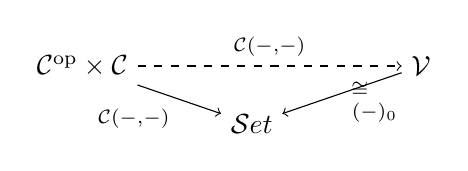
\begin{tikzpicture}[x=1.7em,y=1.4em]
  \node (tl) at (0,1.5) {$\mathcal{C}^{\mathrm{op}}\times\mathcal{C}$};
  \node (tr) at (7.2,1.5) {$\mathcal{V}$};
  \node (b)  at (3.6,0) {$\mathcal{S}et$};
  \draw[->,dashed] (tl) -- node[above]{$\scriptstyle\mathcal{C}(-,-)$} (tr);
  \draw[->] (tl) -- node[below left]{$\scriptstyle\mathcal{C}(-,-)$} (b);
  \draw[->] (tr) -- node[below right]{$\scriptstyle(-)_{0}$} (b);
  \node at (5.9,0.9) {$\scriptstyle\cong$};
\end{tikzpicture}
\end{center}
此外，取值于 $\mathcal{V}$ 中的可表示函子
$\mathcal{C}(-,-)\colon\mathcal{C}^{\mathrm{op}}\times\mathcal{C}\to\mathcal{V}$
必须是\cref{ex:v-bifunctor}意义下的一个 $\mathcal{V}$-二函子，这告诉我们：
复合映射可以在 $\mathcal{V}$ 内部定义，而且恒等定律与结合定律也在那里成立。
\end{remark}

「取底非富集范畴」与「取自由范畴」这两种构造都是函子式的（见%
\cref{ex:underlying-free-functorial}）。这两种构造之间的关系由下述命题概括，
其证明留作练习，因为它被\cref{cor:underlying-free-2-adjunction}所加强。

\begin{proposition}\label{prop:free-v-category-fully-faithful}
自由 $\mathcal{V}$-范畴函子定义底范畴函子的一个\trFullyFaithful{}
\trLeftAdjoint。从而，一个 $\mathcal{V}$-范畴是自由的，恰当时它经由该伴随的
余单位\trIsomorphism{}于其底范畴上的自由范畴。
\end{proposition}

\begin{proof}
\cref{ex:proof-free-v-category-fully-faithful}。
\end{proof}

\subsection*{练习}

\begin{exercise}\label{ex:underlying-category-is-category}
验证\cref{def:underlying-category}所描述的富集范畴之底范畴确实是一个%
\trCategory。
\end{exercise}

\begin{exercise}\label{ex:unit-condition}
验证\cref{lem:cartesian-closed-v-category}之证明中留给读者的那个单位条件。
\end{exercise}

\begin{exercise}\label{ex:opposite-v-category}
定义一个 $\mathcal{V}$-范畴的 \textbf{反者}（opposite），并对偶化%
\cref{exa:enriched-representable}以定义反变的富集可表示函子。
\end{exercise}

\begin{exercise}\label{ex:v-bifunctor}
\begin{enumerate}[label=(\roman*)]
\item 定义两个 $\mathcal{V}$-范畴的 \textbf{笛卡尔积}（cartesian product）。
\item 定义一个 \textbf{多变量 $\mathcal{V}$-函子}（multivariable
  $\mathcal{V}$-functor）。
\item 利用这些概念证明：任何 $\mathcal{V}$-范畴 $\mathcal{C}$ 都配备有一个%
  \trCanonical{} $\mathcal{V}$-二函子
  $\mathcal{C}(-,-)\colon\allowbreak\mathcal{C}^{\mathrm{op}}\times\allowbreak\mathcal{C}\to\allowbreak\mathcal{V}$，
  它限制到协变与反变的可表示函子上。
\end{enumerate}
\end{exercise}

\begin{exercise}\label{ex:underlying-free-functorial}
\begin{enumerate}[label=(\roman*)]
\item 定义一个富集函子的底函子。
\item 证明从富集函子到底非富集函子的过渡是函子式的。
\item 定义一个非富集函子上的自由富集函子。
\item 证明从非富集函子到自由富集函子的过渡是函子式的。
\end{enumerate}
\end{exercise}

\begin{exercise}[A.7.6]\label{ex:proof-free-v-category-fully-faithful}
证明\cref{prop:free-v-category-fully-faithful}。
\end{exercise}

   %

\providecommand{\Cat}{\mathcal{C}at}
\providecommand{\sSet}{s\mathcal{S}et}

\section{富集\trNaturalTransformation{}与富集\trYonedaLemma}\label{sec:enriched-yoneda-lemma}

回忆：平行\trFunctor{} $F,G\colon\mathcal{C}\to\mathcal{D}$ 之间的一个（非富集的）%
\trNaturalTransformation{} $\alpha\colon F\Rightarrow G$ 由下列数据给出：
\begin{itemize}
\item 对每个 $x\in\mathcal{C}$，一条箭头 $\alpha_{x}\in\mathcal{D}(Fx,Gx)$ 的
  数据；
\item 并要求对每个态射 $f\in\mathcal{C}(x,y)$，图表
\begin{rveq}\label{eq:unenriched-naturality-square}
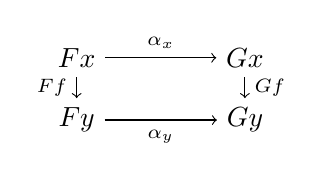
\begin{tikzpicture}[x=1.9em,y=1.5em]
  \node (tl) at (0,1.5) {$Fx$};
  \node (tr) at (3.2,1.5) {$Gx$};
  \node (bl) at (0,0) {$Fy$};
  \node (br) at (3.2,0) {$Gy$};
  \draw[->] (tl) -- node[above]{$\scriptstyle\alpha_{x}$} (tr);
  \draw[->] (tl) -- node[left]{$\scriptstyle Ff$} (bl);
  \draw[->] (tr) -- node[right]{$\scriptstyle Gf$} (br);
  \draw[->] (bl) -- node[below]{$\scriptstyle\alpha_{y}$} (br);
\end{tikzpicture}
\end{rveq}
  在 $\mathcal{D}$ 中交换。
\end{itemize}

这一概念可富集为 $\mathcal{V}$-\trNaturalTransformation{}的概念：其数据恰好
相同——即 $\mathcal{D}$ 的底\trCategory{}中由 $\mathcal{C}$ 的诸对象加标的一族
箭头——但带有一个更强的 $\mathcal{V}$-自然性条件，后者经由把自然性条件
\eqref{eq:unenriched-naturality-square} 内化而得到表达。

\begin{definition}\label{def:vnatural-transformation}
介于 $\mathcal{V}$-富集\trFunctor{} $F,G\colon\mathcal{C}\to\mathcal{D}$ 之间的
$\mathcal{V}$\textbf{-富集\trNaturalTransformation}（$\mathcal{V}$-enriched
natural transformation）或称 $\mathcal{V}$\textbf{-\trNaturalTransformation}
（$\mathcal{V}$-natural transformation）$\alpha\colon F\Rightarrow G$ 由下列
数据给出：
\begin{itemize}
\item 对每个 $x\in\mathcal{C}$，一条箭头 $\alpha_{x}\colon 1\to\mathcal{D}(Fx,Gx)$；
\item 使得对每一对对象 $x$，$y\in\mathcal{C}$，下述 $\mathcal{V}$-自然性方块在
  $\mathcal{V}$ 中交换：
\begin{rveq}\label{eq:vnaturality-square}
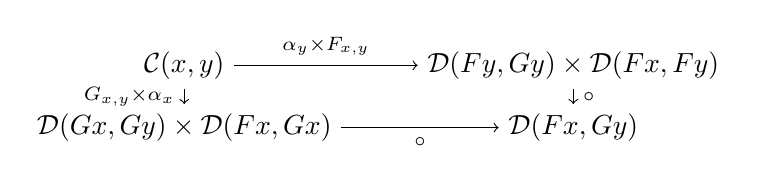
\begin{tikzpicture}[x=1.9em,y=1.5em]
  \node (tl) at (0,1.5) {$\mathcal{C}(x,y)$};
  \node (tr) at (7.4,1.5) {$\mathcal{D}(Fy,Gy)\times\mathcal{D}(Fx,Fy)$};
  \node (bl) at (0,0) {$\mathcal{D}(Gx,Gy)\times\mathcal{D}(Fx,Gx)$};
  \node (br) at (7.4,0) {$\mathcal{D}(Fx,Gy)$};
  \draw[->] (tl) -- node[above]{$\scriptstyle\alpha_{y}\times F_{x,y}$} (tr);
  \draw[->] (tl) -- node[left]{$\scriptstyle G_{x,y}\times\alpha_{x}$} (bl);
  \draw[->] (tr) -- node[right]{$\scriptstyle\circ$} (br);
  \draw[->] (bl) -- node[below]{$\scriptstyle\circ$} (br);
\end{tikzpicture}
\end{rveq}
\end{itemize}
\end{definition}

\begin{example}\label{exa:post-composition-vnatural-transformation}
一个 $\mathcal{V}$-\trCategory{} $\mathcal{C}$ 的底\trCategory{}中的一条箭头
$f\colon 1\to\mathcal{C}(x,y)$ 定义一支 $\mathcal{V}$-\trNaturalTransformation
$-\circ f\colon\mathcal{C}(y,-)\Rightarrow\mathcal{C}(x,-)$——介于诸富集可表示%
\trFunctor{}之间——其在 $z\in\mathcal{C}$ 处的分量由在 $f$ 处对复合映射的伴随转置
求值而定义：
\[ 1\xrightarrow{\ f\ }\mathcal{C}(x,y)
   \xrightarrow{\ \mathcal{C}(-,z)_{x,y}\ }\mathcal{C}(x,z)^{\mathcal{C}(y,z)} \]
所要求的 $\mathcal{V}$-自然性方块，经由对 $\mathcal{C}$ 的结合律图表求一个分量
之值而得到。
\end{example}

$\mathcal{V}$-\trNaturalTransformation{}的复合方式与非富集的%
\trNaturalTransformation{}相同：

\begin{definition}\label{def:vertical-horizontal-composites}
介于 $\mathcal{C}$ 与 $\mathcal{D}$ 之间的 $\mathcal{V}$-\trNaturalTransformation
$\alpha\colon F\Rightarrow G$ 与 $\beta\colon G\Rightarrow H$ 的\textbf{竖直复合}
（vertical composite）$\beta\cdot\alpha$ 在 $x\in\mathcal{C}$ 处的分量
$(\beta\cdot\alpha)_{x}$ 定义为复合
\[ 1\xrightarrow{\ \beta_{x}\times\alpha_{x}\ }
   \mathcal{D}(Gx,Hx)\times\mathcal{D}(Fx,Gx)
   \xrightarrow{\ \circ\ }\mathcal{D}(Fx,Hx) \]
从 $\mathcal{C}$ 到 $\mathcal{D}$ 的 $\alpha\colon F\Rightarrow G$ 与从
$\mathcal{D}$ 到 $\mathcal{E}$ 的 $\gamma\colon H\Rightarrow K$ 的\textbf{水平
复合}（horizontal composite）$\gamma*\alpha$ 在 $x\in\mathcal{C}$ 处的分量
$(\gamma*\alpha)_{x}$ 定义为公共复合
\begin{center}
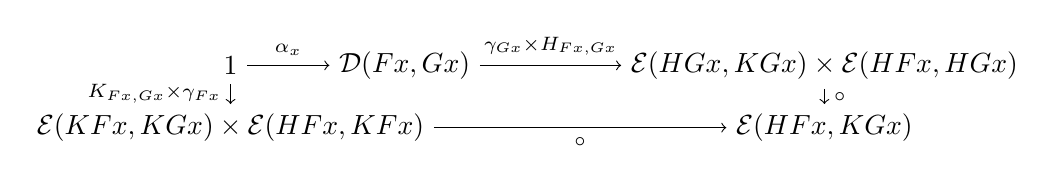
\begin{tikzpicture}[x=1.85em,y=1.5em]
  \node (tl) at (0,1.5) {$1$};
  \node (tm) at (3.4,1.5) {$\mathcal{D}(Fx,Gx)$};
  \node (tr) at (11.6,1.5) {$\mathcal{E}(HGx,KGx)\times\mathcal{E}(HFx,HGx)$};
  \node (bl) at (0,0) {$\mathcal{E}(KFx,KGx)\times\mathcal{E}(HFx,KFx)$};
  \node (br) at (11.6,0) {$\mathcal{E}(HFx,KGx)$};
  \draw[->] (tl) -- node[above]{$\scriptstyle\alpha_{x}$} (tm);
  \draw[->] (tm) -- node[above]{$\scriptstyle\gamma_{Gx}\times H_{Fx,Gx}$} (tr);
  \draw[->] (tl) -- node[left]{$\scriptstyle K_{Fx,Gx}\times\gamma_{Fx}$} (bl);
  \draw[->] (tr) -- node[right]{$\scriptstyle\circ$} (br);
  \draw[->] (bl) -- node[below]{$\scriptstyle\circ$} (br);
\end{tikzpicture}
\end{center}
它由 $\gamma$ 的 $\mathcal{V}$-自然性给出良定义。\footnote{原书此图右上节点
印作「$\mathcal{E}(KGx,HGx)\times\mathcal{E}(HFx,HGx)$」，按公共复合之型两
因子次序倒置；右下节点花体印作「$\mathcal{D}(HFx,KGx)$」，$\mathcal{D}$ 疑为
$\mathcal{E}$ 之误；均径改。——译者注}这些构造的 $\mathcal{V}$-自然性
留作\cref{ex:vertical-horizontal-vnatural}。
\end{definition}

一支 $\mathcal{V}$-\trNaturalTransformation{}的\textbf{底自然变换}（underlying
natural transformation）由同一族箭头给出。非富集的自然性条件
\eqref{eq:unenriched-naturality-square} 经由在一条底箭头
$f\colon 1\to\mathcal{C}(x,y)$ 处对富集自然性条件
\eqref{eq:vnaturality-square} 求值而得到。特别地，$\mathcal{V}$-%
\trNaturalTransformation{}的竖直复合与水平复合的中间四项交换规则（见附录 B 中的%
\cref{def:two-category}）由非富集\trNaturalTransformation{}的竖直复合与水平复合的中间四项交换
规则推得，盖因后者的数据决定前者的数据。从而，%
\cref{ex:vertical-horizontal-vnatural} 蕴含：

\begin{corollary}\label{cor:vcat-two-category}
对任何\trCartesianClosed{}\trCategory{} $\mathcal{V}$，存在一个由 $\mathcal{V}$-%
\trCategory、$\mathcal{V}$-\trFunctor{}与 $\mathcal{V}$-\trNaturalTransformation{}%
组成的 2-\trCategory{} $\mathcal{V}\text{-}\Cat$。
\end{corollary}

我们如今将注意力转向 $\mathcal{V}$-富集\trYonedaLemma，我们将以若干形式陈述之。
\trYonedaLemma{}的一个角色，是给出 $\mathcal{C}$ 中同构对象的一个可表示刻画。当
$\mathcal{C}$ 是一个 $\mathcal{V}$-\trCategory{}时，这有若干形式。下述结果中所
谈及的 $\mathcal{V}$\textbf{-自然同构}（$\mathcal{V}$-natural isomorphism）
概念，定义为一支带有关于竖直复合之逆 $\alpha^{-1}\colon G\Rightarrow F$ 的
$\mathcal{V}$-\trNaturalTransformation{} $\alpha\colon F\Rightarrow G$。

\begin{lemma}\label{lem:isomorphism-characterizations}
对 $\mathcal{V}$-\trCategory{} $\mathcal{C}$ 中的对象 $x$ 与 $y$，下述诸款等价：
\begin{enumerate}[label=(\roman*)]
\item $x$ 与 $y$ 作为 $\mathcal{C}$ 的底\trCategory{}的对象是同构的。
\item 取值于 $\mathcal{S}et$ 的诸非富集可表示函子
  $\mathcal{C}(x,-),\mathcal{C}(y,-)\colon\mathcal{C}\to\mathcal{S}et$ 是自然
  同构的。
\item 取值于 $\mathcal{V}$ 的诸非富集可表示函子
  $\mathcal{C}(x,-),\mathcal{C}(y,-)\colon\mathcal{C}\to\mathcal{V}$ 是自然
  同构的。
\item 取值于 $\mathcal{V}$ 的诸 $\mathcal{V}$-\trFunctor{}
  $\mathcal{C}(x,-),\mathcal{C}(y,-)\colon\mathcal{C}\to\mathcal{V}$ 是
  $\mathcal{V}$-自然同构的。
\end{enumerate}
\end{lemma}

\begin{proof}
应用底范畴 2-\trFunctor{} $(-)_{0}\colon\mathcal{V}\text{-}\Cat\to\Cat$，第四款
蕴含第三款。第三款经由与底集函子 $(-)_{0}\colon\mathcal{V}\to\mathcal{S}et$ 作%
\trWhiskering{}而蕴含第二款。第二款由非富集的\trYonedaLemma{}蕴含第一款；这仍是
要点所在。最后，第一款经由一个直接构造蕴含第四款：若
$f\colon 1\to\mathcal{C}(x,y)$ 与 $g\colon 1\to\mathcal{C}(y,x)$ 在 $\mathcal{C}$
的底\trCategory{}中定义一个\trIsomorphism，则%
\cref{exa:post-composition-vnatural-transformation}中相应的可表示
$\mathcal{V}$-\trNaturalTransformation{}定义一个 $\mathcal{V}$-自然同构。
\end{proof}

\cref{lem:isomorphism-characterizations}定义了富集\trCategory{}的两对象之间的一个
常见的\textbf{\trIsomorphism}概念，而这一概念最终与通常非富集的同构概念并无
不同。这可以视为定义了富集\trYonedaLemma{}的一种「廉价」形式。$\mathcal{V}$-%
\trYonedaLemma{}的完全形式将通常的陈述——介于「定义域为一支可表示\trFunctor{}的
那些\trNaturalTransformation{}所成之集」与「由在表示对象处对陪域求值所定义之集」
之间的一个自然\trIsomorphism——富集为 $\mathcal{V}$ 中的一个\trIsomorphism。
使之精确的第一步，是将一对平行 $\mathcal{V}$-\trFunctor{}之间的
$\mathcal{V}$-\trNaturalTransformation{}之集富集为 $\mathcal{V}$ 的一个对象。

\begin{definition}\label{def:vobject-natural-transformations}
设 $\mathcal{V}$ 是一个\trComplete{}\trCartesianClosed{}\trCategory，并考虑
$\mathcal{V}$-\trFunctor{}的一个平行对 $F,G\colon\mathcal{C}\to\mathcal{D}$，其中
$\mathcal{C}$ 是一个小 $\mathcal{V}$-\trCategory。于是，
$\mathcal{V}$\textbf{-\trNaturalTransformation{}对象}（$\mathcal{V}$-object of
$\mathcal{V}$-natural transformations）由等化子图表（equalizer diagram）
\[ \mathcal{D}^{\mathcal{C}}(F,G)\longrightarrow
   \prod_{z\in\mathcal{C}}\mathcal{D}(Fz,Gz)
   \;\rightrightarrows\;
   \prod_{x,y\in\mathcal{C}}\mathcal{D}(Fx,Gy)^{\mathcal{C}(x,y)} \]
定义，其中等化子图表中指向 $\mathcal{D}(Fx,Gy)^{\mathcal{C}(x,y)}$ 的两个映射，
一个由投射到 $\mathcal{D}(Fx,Gx)$、施加 $G$ 在箭头上的内部作用（internal
action）、然后再复合而定义，另一个则由投射到 $\mathcal{D}(Fy,Gy)$、施加 $F$ 在
箭头上的内部作用、然后再复合而定义：
\begin{center}
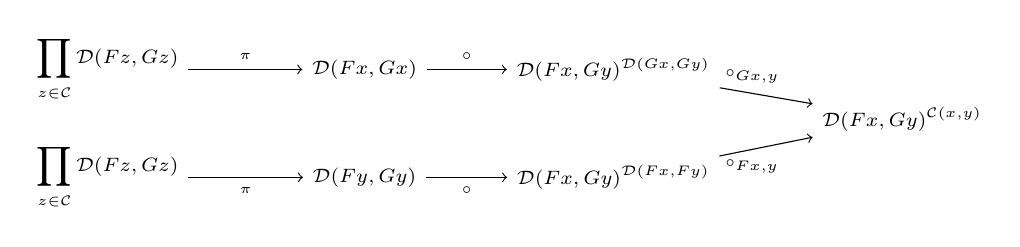
\begin{tikzpicture}[x=1.45em,y=1.5em,every node/.style={font=\scriptsize}]
  \node (pl) at (0,1.5) {$\displaystyle\prod_{z\in\mathcal{C}}\mathcal{D}(Fz,Gz)$};
  \node (t1) at (6.4,1.5) {$\mathcal{D}(Fx,Gx)$};
  \node (t2) at (12.6,1.5) {$\mathcal{D}(Fx,Gy)^{\mathcal{D}(Gx,Gy)}$};
  \node (r)  at (19.8,0.3) {$\mathcal{D}(Fx,Gy)^{\mathcal{C}(x,y)}$};
  \node (bl) at (0,-1.1) {$\displaystyle\prod_{z\in\mathcal{C}}\mathcal{D}(Fz,Gz)$};
  \node (b1) at (6.4,-1.1) {$\mathcal{D}(Fy,Gy)$};
  \node (b2) at (12.6,-1.1) {$\mathcal{D}(Fx,Gy)^{\mathcal{D}(Fx,Fy)}$};
  \draw[->] (pl) -- node[above]{$\scriptstyle\pi$} (t1);
  \draw[->] (t1) -- node[above]{$\scriptstyle\circ$} (t2);
  \draw[->] (t2) -- node[above,pos=0.35]{$\scriptstyle\circ_{Gx,y}$} (r);
  \draw[->] (bl) -- node[below]{$\scriptstyle\pi$} (b1);
  \draw[->] (b1) -- node[below]{$\scriptstyle\circ$} (b2);
  \draw[->] (b2) -- node[below,pos=0.35]{$\scriptstyle\circ_{Fx,y}$} (r);
\end{tikzpicture}
\end{center}
\end{definition}

\begin{lemma}\label{lem:underlying-set-of-vobject}
$\mathcal{V}$-\trNaturalTransformation{}对象
$\mathcal{V}^{\mathcal{C}}(F,G)$ 的底集，是从 $F$ 到 $G$ 的
$\mathcal{V}$-\trNaturalTransformation{}之集。
\end{lemma}

\begin{proof}
由其定义性的\trUniversalProperty，$\mathcal{V}^{\mathcal{C}}(F,G)$ 底集的诸%
\trElement{}对应于使\cref{def:vobject-natural-transformations}所述的平行映射对
等化的那些映射 $\alpha\colon 1\to\prod_{z\in\mathcal{C}}\mathcal{V}(Fz,Gz)$。
该映射 $\alpha$ 定义一支 $\mathcal{V}$-\trNaturalTransformation{}
$\alpha\colon F\Rightarrow G$ 的诸分量，而交换性条件转置后恰为
\eqref{eq:vnaturality-square}。
\end{proof}

\trYonedaLemma{}可以由「在恒同处求值是一个同构」这句口号来表达；但由于在富集情境
中，\trNaturalTransformation{}的富集对象是经由一个\trLimit{}定义的，较为容易的
做法是转而定义诱导出\trNaturalTransformation{}的那个映射。给定小
$\mathcal{V}$-\trCategory{} $\mathcal{A}$ 中的一个对象 $a\in\mathcal{A}$ 与一支
$\mathcal{V}$-\trFunctor{} $F\colon\mathcal{A}\to\mathcal{V}$，$F$ 在箭头上的内部
作用经转置而定义一个使平行对
\begin{rveq}\label{eq:internal-action-parallel-pair}
Fa\overset{F_{a,-}}{\dashrightarrow}\prod_{z\in\mathcal{A}}Fz^{\mathcal{A}(a,z)}
\;\rightrightarrows\;
\prod_{x,y\in\mathcal{A}}Fy^{\mathcal{A}(a,x)\times\mathcal{A}(x,y)}
\end{rveq}
等化的映射，从而在 $\mathcal{V}$ 中诱导一个典范映射
$Fa\to\mathcal{V}^{\mathcal{A}}(\mathcal{A}(a,-),F)$。

\begin{theorem}[富集\trYonedaLemma]\label{thm:enriched-yoneda}
对任何小 $\mathcal{V}$-\trCategory{} $\mathcal{A}$、对象 $a\in\mathcal{A}$ 与一支
$\mathcal{V}$-\trFunctor{} $F\colon\mathcal{A}\to\mathcal{V}$，该典范映射定义
$\mathcal{V}$ 中的一个\trIsomorphism
\[ Fa\simeq\mathcal{V}^{\mathcal{A}}(\mathcal{A}(a,-),F) \]
且该\trIsomorphism{}在 $a$ 与 $F$ 二者中都是 $\mathcal{V}$-自然的。
\end{theorem}

\begin{proof}
为证该\trIsomorphism，只需验证 \eqref{eq:internal-action-parallel-pair} 是一个%
\trLimit{}锥。为此，考虑该平行对上的另一个锥
\[ \nu\xrightarrow{\ \lambda\ }\prod_{z\in\mathcal{A}}Fz^{\mathcal{A}(a,z)}
   \;\rightrightarrows\;
   \prod_{x,y\in\mathcal{A}}Fy^{\mathcal{A}(a,x)\times\mathcal{A}(x,y)} \]
并经由在 $\mathrm{id}_{a}$ 处对分量 $\lambda_{a}$ 的转置求值而定义一个候选的因子
分解：
\[ \lambda_{a}(\mathrm{id}_{a})\coloneqq\nu
   \xrightarrow{\ \mathrm{id}_{a}\times\nu\ }\mathcal{A}(a,a)\times\nu
   \xrightarrow{\ \lambda_{a}\ }Fa \]
为证 $\lambda_{a}(\mathrm{id}_{a})\colon\nu\to Fa$ 确实定义 $\lambda$ 穿过该%
\trLimit{}锥的一个因子分解，只需在该乘积的每个分量 $Fz^{\mathcal{A}(a,z)}$ 处
证明交换性，我们以转置的形式验证之：
\begin{center}
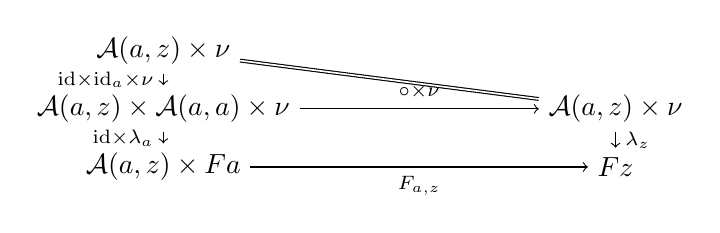
\begin{tikzpicture}[x=1.9em,y=1.4em]
  \node (t)  at (0,3.0) {$\mathcal{A}(a,z)\times\nu$};
  \node (ml) at (0,1.5) {$\mathcal{A}(a,z)\times\mathcal{A}(a,a)\times\nu$};
  \node (mr) at (8.6,1.5) {$\mathcal{A}(a,z)\times\nu$};
  \node (bl) at (0,0) {$\mathcal{A}(a,z)\times Fa$};
  \node (br) at (8.6,0) {$Fz$};
  \draw[->] (t) -- node[left]{$\scriptstyle\mathrm{id}\times\mathrm{id}_{a}\times\nu$} (ml);
  \draw[double] (t) -- (mr);
  \draw[->] (ml) -- node[above]{$\scriptstyle\circ\times\nu$} (mr);
  \draw[->] (ml) -- node[left]{$\scriptstyle\mathrm{id}\times\lambda_{a}$} (bl);
  \draw[->] (mr) -- node[right]{$\scriptstyle\lambda_{z}$} (br);
  \draw[->] (bl) -- node[below]{$\scriptstyle F_{a,z}$} (br);
\end{tikzpicture}
\end{center}
上方三角形由 $\mathcal{A}$ 的恒等律而交换，而下方方块之所以交换，是因为
$\lambda$ 定义平行对上的一个锥。因子分解 $\lambda_{a}(\mathrm{id}_{a})$ 的唯一
性由同一图表沿 $z=a$ 取值并在 $\mathrm{id}_{a}$ 处求值而推得。
$Fa\cong\mathcal{V}^{\mathcal{A}}(\mathcal{A}(a,-),F)$ 之 $\mathcal{V}$-自然性的
验证留给读者，或见文献 \cite[\S 2.4]{bib68}。
\end{proof}

过渡到底集：

\begin{corollary}\label{cor:yoneda-bijection}
对任何小 $\mathcal{V}$-\trCategory{} $\mathcal{A}$、对象 $a\in\mathcal{A}$ 与一支
$\mathcal{V}$-\trFunctor{} $F\colon\mathcal{A}\to\mathcal{V}$，在
$\mathcal{V}$-\trNaturalTransformation{} $\alpha\colon\mathcal{A}(a,-)\Rightarrow F$
与 $Fa$ 的底集中的诸\trElement{} $u\colon 1\to Fa$ 之间存在一个自然双射，后者由在
$a\in\mathcal{A}$ 处的分量于恒同 $\mathrm{id}_{a}$ 处求值而实现。
\end{corollary}

这就给出了一个证成 $\mathcal{V}$-\trFunctor{}之可表示性的判据：呈现确立定义性
$\mathcal{V}$-自然同构所需的最小数据即可。

\begin{corollary}\label{cor:represent-functor}
对一支 $\mathcal{V}$-\trFunctor{}
$F\colon\mathcal{A}^{\mathrm{op}}\to\mathcal{V}$ 与一个对象 $a\in\mathcal{A}$，
下述诸款等价，且它们定义「$a$ \textbf{表示}（represent）$F$」之所指：
\begin{enumerate}[label=(\roman*)]
\item 存在 $\mathcal{V}$ 中的一个\trIsomorphism{} $\mathcal{A}(x,a)\cong Fx$，
  其在 $x\in\mathcal{A}$ 中是 $\mathcal{V}$-自然的。
\item 存在 $Fa$ 的底集中的一个\trElement{} $u\colon 1\to Fa$，使得复合映射
\[ \mathcal{A}(x,a)\xrightarrow{\ F_{x,a}\ }\mathcal{V}(Fa,Fx)
   \xrightarrow{\ \circ u\ }\mathcal{V}(1,Fx)\cong Fx \]
  对一切 $x\in\mathcal{A}$ 都定义 $\mathcal{V}$ 中的一个\trIsomorphism。
\end{enumerate}
\end{corollary}

\begin{proof}
由\cref{cor:yoneda-bijection}，$Fa$ 底集中的\trElement{} $u\colon 1\to Fa$ 决定
一支唯一的 $\mathcal{V}$-\trNaturalTransformation{}
$\mathcal{A}(-,a)\Rightarrow F$，其在 $x\in\mathcal{A}$ 处的分量即陈述中的那个
映射。于是，泛\trElement{} $u$ 定义一个 $\mathcal{V}$-自然同构而不只是一支
$\mathcal{V}$-\trNaturalTransformation，恰当陈述中的那个映射是\trIsomorphism{}%
之时。
\end{proof}

既然我们已经假定富集之基是\trCartesianClosed，2-\trCategory{}
$\mathcal{V}\text{-}\Cat$ 便容许有限\trProduct，这使得我们能够定义多变量
$\mathcal{V}$-\trFunctor（见\cref{ex:v-bifunctor}）。下述结果蕴含：在 A.4 节与 A.5 节中由
$\mathcal{V}$-自然同构所刻画的那些结构可以拼装成 $\mathcal{V}$-\trFunctor。

\begin{proposition}\label{prop:unique-extension-vfunctor}
设 $M\colon\mathcal{B}^{\mathrm{op}}\times\mathcal{A}\to\mathcal{V}$ 是一支
$\mathcal{V}$-\trFunctor，使得对每个 $a\in\mathcal{A}$，$\mathcal{V}$-%
\trFunctor{} $M(-,a)\colon\mathcal{B}^{\mathrm{op}}\to\mathcal{V}$ 被某个
$Fa\in\mathcal{B}$ 所表示，意即存在一个 $\mathcal{V}$-自然\trIsomorphism
\[ \mathcal{B}(b,Fa)\cong M(b,a). \]
那么，存在唯一的方式把映射 $a\in\mathcal{A}\mapsto Fa\in\mathcal{B}$ 扩张为一支
$\mathcal{V}$-\trFunctor{} $F\colon\mathcal{A}\to\mathcal{B}$，使得诸%
\trIsomorphism{}在 $a\in\mathcal{A}$ 中以及在 $b\in\mathcal{B}$ 中都是
$\mathcal{V}$-自然的。
\end{proposition}

\begin{proof}
由\cref{cor:yoneda-bijection}之形式的\trYonedaLemma，对每个 $a\in\mathcal{A}$
定义一族在 $b\in\mathcal{B}$ 中 $\mathcal{V}$-自然的\trIsomorphism{}
$\alpha_{b,a}\colon\mathcal{B}(b,Fa)\cong M(b,a)$，就等于对每个
$a\in\mathcal{A}$ 定义一族满足\cref{cor:represent-functor}(ii)之条件的%
\trElement{} $\eta_{a}\colon 1\to M(Fa,a)$。由\trYonedaLemma{}中的
$\mathcal{V}$-自然性陈述，\trIsomorphism{} $\alpha_{b,a}$ 在 $a$ 中为
$\mathcal{V}$-自然，等价于\trElement{}之族 $\eta_{a}\colon 1\to M(Fa,a)$ 在 $a$
中「超自然地」$\mathcal{V}$-自然。这意味着：对任何一对对象
$a$，$a'\in\mathcal{A}$，外侧方块交换：
\begin{center}
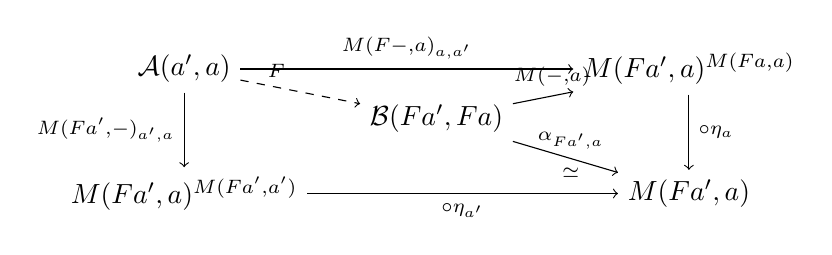
\begin{tikzpicture}[x=1.9em,y=1.5em]
  \node (tl) at (0,3.0) {$\mathcal{A}(a',a)$};
  \node (tr) at (9.6,3.0) {$M(Fa',a)^{M(Fa,a)}$};
  \node (c)  at (4.8,1.8) {$\mathcal{B}(Fa',Fa)$};
  \node (bl) at (0,0) {$M(Fa',a)^{M(Fa',a')}$};
  \node (br) at (9.6,0) {$M(Fa',a)$};
  \draw[->] (tl) -- node[above]{$\scriptstyle M(F-,a)_{a,a'}$} (tr);
  \draw[->,dashed] (tl) -- node[above,pos=0.3]{$\scriptstyle F$} (c);
  \draw[->] (c) -- node[above,pos=0.65]{$\scriptstyle M(-,a)$} (tr);
  \draw[->] (tl) -- node[left]{$\scriptstyle M(Fa',-)_{a',a}$} (bl);
  \draw[->] (tr) -- node[right]{$\scriptstyle\circ\eta_{a}$} (br);
  \draw[->] (bl) -- node[below]{$\scriptstyle\circ\eta_{a'}$} (br);
  \draw[->] (c) -- node[above,pos=0.55]{$\scriptstyle\alpha_{Fa',a}$}
    node[below,pos=0.55]{$\scriptstyle\simeq$} (br);
\end{tikzpicture}
\end{center}
正如上方三角形所展示的，顶行映射 $M(F-,a)_{a',a}$ 穿过 $F$ 在箭头上的、我们所要
定义的那个内部作用而分解；但请注意，如右方三角形所示，另一因子与右侧竖直映射的
复合正是自然\trIsomorphism{} $\alpha_{Fa',a}$。于是，存在唯一的方式定义
$F_{a',a}$ 使超自然的 $\mathcal{V}$-自然性方块交换——亦即通过保证左下四边形
交换，而这正是所要的断言。$F$ 的这些内部作用映射的 $\mathcal{V}$-函子性由 $M$
在 $\mathcal{A}$ 变量中的 $\mathcal{V}$-函子性推得。
\end{proof}

我们以富集\trYonedaLemma{}的若干应用来结束本节。$\mathcal{V}$-富集\trEquivalence
或 $\mathcal{V}$-富集\trAdjunction{}的正确概念，由在 2-\trCategory{}
$\mathcal{V}\text{-}\Cat$ 中诠释等价与伴随的标准 2-范畴论概念而给出。为作对比，
我们在此以另一种形式呈现这两个概念，并留给读者去应用\cref{thm:enriched-yoneda}
将它们与 2-范畴论概念联系起来。

\begin{definition}\label{def:vequivalent}
一对 $\mathcal{V}$-\trCategory{} $\mathcal{C}$ 与 $\mathcal{D}$ 是
$\mathcal{V}$-\textbf{\trEquivalence}的（$\mathcal{V}$-equivalent），若存在一支
$\mathcal{V}$-\trFunctor{} $F\colon\mathcal{C}\to\mathcal{D}$，它
\begin{itemize}
\item 是 $\mathcal{V}$-\textbf{\trFullyFaithful}：每个
  $F_{x,y}\colon\mathcal{C}(x,y)\to\mathcal{D}(Fx,Fy)$ 都是 $\mathcal{V}$ 中的
  一个\trIsomorphism；并且
\item 在对象上\trEssentiallySurjective：每个 $d\in\mathcal{D}$ 都同构于某个
  $c\in\mathcal{C}$ 的 $Fc$。
\end{itemize}
\end{definition}

\begin{definition}\label{def:vadjunction}
一个 $\mathcal{V}$\textbf{-\trAdjunction}（$\mathcal{V}$-adjunction）由一对
$\mathcal{V}$-\trFunctor{} $F\colon\mathcal{B}\to\mathcal{A}$ 与
$U\colon\mathcal{A}\to\mathcal{B}$ 连同诸\trIsomorphism
\[ \mathcal{A}(Fb,a)\cong\mathcal{B}(b,Ua) \]
给出，后者在 $a\in\mathcal{A}$ 与 $b\in\mathcal{B}$ 二者中都是 $\mathcal{V}$-%
自然的。
\end{definition}

\begin{remark}\label{rem:vleft-adjoint-representability}
由\cref{prop:unique-extension-vfunctor}，一支 $\mathcal{V}$-\trFunctor{}
$U\colon\mathcal{A}\to\mathcal{B}$ 容有一个 $\mathcal{V}$-\trLeftAdjoint，当且
仅当每个 $\mathcal{B}(b,U-)\colon\mathcal{A}\to\mathcal{V}$ 被某个对象
$Fb\in\mathcal{A}$ 所表示；此时，$\mathcal{V}$-自然\trIsomorphism{}
$\mathcal{A}(Fb,-)\cong\mathcal{B}(b,U-)$ 的数据便赋予
$b\in\mathcal{B}\mapsto Fb\in\mathcal{A}$ 以一支 $\mathcal{V}$-\trFunctor{}的
结构。对偶的注可为一支给定的 $\mathcal{V}$-\trFunctor{}构造富集%
\trRightAdjoint。
\end{remark}

\subsection*{练习}

\begin{exercise}\label{ex:vertical-horizontal-vnatural}
验证\cref{def:vertical-horizontal-composites}中的竖直复合与水平复合是
$\mathcal{V}$-自然的。
\end{exercise}

\begin{exercise}\label{ex:functor-arrow-vnatural}
设 $F\colon\mathcal{C}\to\mathcal{D}$ 是一支 $\mathcal{V}$-\trFunctor。证明映射
\[ \mathcal{C}(x,y)\xrightarrow{\ F_{x,y}\ }\mathcal{D}(Fx,Fy) \]
在 $x$ 与 $y$ 二者中都是 $\mathcal{V}$-自然的。
\end{exercise}

\begin{exercise}\label{ex:functor-category-vcategory}
在 $\mathcal{V}$ \trComplete{}情形下，证明：对任何一对 $\mathcal{V}$-%
\trCategory{} $\mathcal{C}$ 与 $\mathcal{D}$（其中 $\mathcal{C}$ 小），%
\cref{def:vobject-natural-transformations}使 $\mathcal{D}^{\mathcal{C}}$ 成为一个
$\mathcal{V}$-\trCategory。
\end{exercise}

\begin{exercise}\label{ex:yoneda-vnaturality}
验证\cref{thm:enriched-yoneda}中的 $\mathcal{V}$-自然性陈述。
\end{exercise}

\begin{exercise}\label{ex:vequivalence-vadjunction-2category}
用\cref{cor:yoneda-bijection}证明：\cref{def:vequivalent}与%
\cref{def:vadjunction}中所给的 $\mathcal{V}$-等价与 $\mathcal{V}$-%
\trAdjunction{}概念，等价于 $\mathcal{V}\text{-}\Cat$ 中的 2-范畴论概念。
\end{exercise}

   %

\section{\trTensor{}与\trCotensor}\label{sec:tensors-and-cotensors}

一个 $\mathcal{V}$-范畴 $\mathcal{C}$ 容有\emph{张量}（tensors），恰当时对一切
$c\in\mathcal{C}$，协变可表示函子
$\mathcal{C}(c,-)\colon\mathcal{C}\to\mathcal{V}$ 容有一个左 $\mathcal{V}$-伴随
$-\otimes c\colon\mathcal{V}\to\mathcal{C}$。对偶地，一个 $\mathcal{V}$-范畴
$\mathcal{C}$ 容有\emph{余张量}（cotensors），恰当时反变可表示函子
$\mathcal{C}(-,c)\colon\mathcal{C}^{\mathrm{op}}\to\mathcal{V}$ 容有一个与之
互为右 $\mathcal{V}$-伴随
$c^{-}\colon\mathcal{V}^{\mathrm{op}}\to\mathcal{C}$。本节的目标是把这两种构造
形式化地引入。我们将会发现，当把诸富集范畴的诸底范畴之间的诸\trFunctor{}加以
富集时，张量或余张量的存在是有用的。

\begin{definition}\label{def:cotensored}
一个 $\mathcal{V}$-范畴 $\mathcal{C}$ 是\textbf{余张量化的}（cotensored），若
对一切 $v\in\mathcal{V}$ 与 $c\in\mathcal{C}$，$\mathcal{V}$-函子
$\mathcal{C}(-,c)^{v}\colon\mathcal{C}^{\mathrm{op}}\to\mathcal{V}$ 被一个对象
$c^{v}\in\mathcal{C}$ 所表示，意即存在一个\trIsomorphism
\[ \mathcal{C}(x,c^{v})\cong\mathcal{C}(x,c)^{v} \]
居于 $\mathcal{V}$ 之中并且在 $x$ 上是 $\mathcal{V}$-自然的。由\cref{prop:unique-extension-vfunctor}，
余张量积定义一个唯一的 $\mathcal{V}$-函子
\[ \mathcal{C}\times\mathcal{V}^{\mathrm{op}}
   \xrightarrow{\ (-)^{-}\ }\mathcal{C} \]
使得定义性\trIsomorphism{}在所有三个变量上都是 $\mathcal{V}$-自然的。
\end{definition}

\begin{definition}\label{def:tensored}
对偶地，一个 $\mathcal{V}$-范畴 $\mathcal{C}$ 是\textbf{张量化的}
（tensored），若对一切 $v\in\mathcal{V}$ 与 $c\in\mathcal{C}$，$\mathcal{V}$-函子
$\mathcal{C}(c,-)^{v}\colon\mathcal{C}\to\mathcal{V}$ 被一个对象
$v\otimes c\in\mathcal{C}$ 所表示，意即存在一个\trIsomorphism
\[ \mathcal{C}(v\otimes c,x)\cong\mathcal{C}(c,x)^{v} \]
居于 $\mathcal{V}$ 之中并且在 $x$ 上是 $\mathcal{V}$-自然的。由\cref{prop:unique-extension-vfunctor}，
\trTensorProduct{}定义一个唯一的 $\mathcal{V}$-函子
\[ \mathcal{V}\times\mathcal{C}\xrightarrow{\ -\otimes-\ }\mathcal{C} \]
使得定义性\trIsomorphism{}在所有三个变量上都是 $\mathcal{V}$-自然的。
\end{definition}

直接从这些定义可得：

\begin{lemma}\label{lem:tensored-cotensored-two-variable-adjunction}
一个 $\mathcal{V}$-范畴 $\mathcal{C}$ 是张量化且余张量化的，当且仅当
$\mathcal{V}$-函子
$\mathcal{C}(-,-)\colon\mathcal{C}^{\mathrm{op}}\times\allowbreak\mathcal{C}\to\allowbreak\mathcal{V}$
参与一个双变量 $\mathcal{V}$-伴随
\[
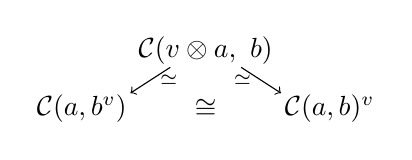
\begin{tikzpicture}[x=1.6em,y=1.5em]
  \node (t)  at (2.8,1.4) {$\mathcal{C}(v\otimes a,\ b)$};
  \node (bl) at (0,0)   {$\mathcal{C}(a,b^{v})$};
  \node (br) at (5.6,0) {$\mathcal{C}(a,b)^{v}$};
  \draw[->] (2.0,1.0) -- node[right]{$\scriptstyle\simeq$} (1.1,0.38);
  \draw[->] (3.6,1.0) -- node[left]{$\scriptstyle\simeq$} (4.5,0.38);
  \node at (2.8,0) {$\cong$};
\end{tikzpicture}
\]
一如这个由 $\mathcal{V}$-自然\trIsomorphism{}组成的交换三角形所表达。%
\footnote{原书此处三角形顶点印作「$\mathcal{C}(v\times a,\ b)$」；按
$v\in\mathcal{V}$、$a\in\mathcal{C}$，笛卡尔积不合型，依定义 A.4.2 之张量
同构 $\mathcal{C}(v\otimes c,x)\cong\mathcal{C}(c,x)^{v}$，疑为张量
$v\otimes a$ 之误，此处径改。——译者注}
\end{lemma}

定义性自然\trIsomorphism{}的 $\mathcal{V}$-自然性有如下推论：

\begin{lemma}\label{lem:tensor-cotensor-unit-associativity}
在任何富集于 $\mathcal{V}$ 之上且余张量化的\trCategory{} $\mathcal{C}$ 中，
存在 $\mathcal{V}$-自然\trIsomorphism
\[ c^{1}\cong c
   \qquad\text{以及}\qquad
   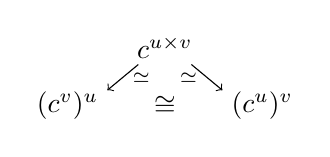
\begin{tikzpicture}[x=1.6em,y=1.5em]
     \node (t)  at (2.2,1.4) {$c^{u\times v}$};
     \node (bl) at (0,0)   {$(c^{v})^{u}$};
     \node (br) at (4.4,0) {$(c^{u})^{v}$};
     \draw[->] (1.6,1.0) -- node[right]{$\scriptstyle\simeq$} (0.9,0.38);
     \draw[->] (2.8,1.0) -- node[left]{$\scriptstyle\simeq$} (3.5,0.38);
     \node at (2.2,0) {$\cong$};
   \end{tikzpicture} \]
对 $u,v\in\mathcal{V}$ 与 $c\in\mathcal{C}$。对偶地，若 $\mathcal{C}$ 富集于
$\mathcal{V}$ 之上且是张量化的，则存在 $\mathcal{V}$-自然\trIsomorphism
\[ 1\otimes c\cong c
   \qquad\text{以及}\qquad
   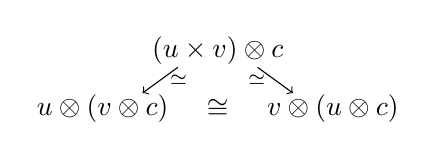
\begin{tikzpicture}[x=1.6em,y=1.5em]
     \node (t)  at (2.6,1.4) {$(u\times v)\otimes c$};
     \node (bl) at (0,0)   {$u\otimes(v\otimes c)$};
     \node (br) at (5.2,0) {$v\otimes(u\otimes c)$};
     \draw[->] (1.7,1.0) -- node[right]{$\scriptstyle\simeq$} (0.9,0.38);
     \draw[->] (3.5,1.0) -- node[left]{$\scriptstyle\simeq$} (4.3,0.38);
     \node at (2.6,0) {$\cong$};
   \end{tikzpicture} \]
对 $u,v\in\mathcal{V}$ 与 $c\in\mathcal{C}$。
\end{lemma}

在这些 $\mathcal{V}$-自然\trIsomorphism{}之间存在种种相干关系，它们源自%
\trCartesianClosed{}\trCategory{} $\mathcal{V}$ 的诸相干关系。

\begin{proof}
由\cref{lem:isomorphism-characterizations}，为定义所显示的那些\trIsomorphism，只需证明这些对象表示同一个
$\mathcal{V}$-函子 $\mathcal{C}^{\mathrm{op}}\to\mathcal{V}$。由余张量的定义性%
\trUniversalProperty，对任何 $x\in\mathcal{C}$，存在 $\mathcal{V}$-自然%
\trIsomorphism
\[ \mathcal{C}(x,c^{1})\cong\mathcal{C}(x,c)^{1}\cong\mathcal{C}(x,c), \]
最后一个\trIsomorphism{}由注 A.1.9（\cref{rem:exponent-one-identity}）给出。
由于这些\trIsomorphism{}在 $c$ 上与在 $x$ 上一样是 $\mathcal{V}$-自然的，
\trIsomorphism{} $c^{1}\cong c$ 也是 $\mathcal{V}$-自然的。

类似地，在下方三角形的三个顶点处各存在 $\mathcal{V}$-自然\trIsomorphism
\begin{center}
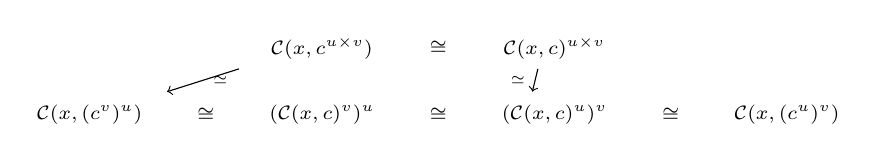
\begin{tikzpicture}[x=1.0em,y=1.5em,every node/.style={font=\scriptsize}]
  \node (T1) at (8.4,1.6) {$\mathcal{C}(x,c^{u\times v})$};
  \node at (12.6,1.6) {$\cong$};
  \node (T2) at (16.8,1.6) {$\mathcal{C}(x,c)^{u\times v}$};
  \node (B1) at (0,0) {$\mathcal{C}(x,(c^{v})^{u})$};
  \node at (4.2,0) {$\cong$};
  \node (B2) at (8.4,0) {$(\mathcal{C}(x,c)^{v})^{u}$};
  \node at (12.6,0) {$\cong$};
  \node (B3) at (16.8,0) {$(\mathcal{C}(x,c)^{u})^{v}$};
  \node at (21.0,0) {$\cong$};
  \node (B4) at (25.2,0) {$\mathcal{C}(x,(c^{u})^{v})$};
  \draw[->] (5.4,1.1) -- node[right]{$\scriptstyle\simeq$} (2.8,0.55);
  \draw[->] (16.2,1.1) -- node[left]{$\scriptstyle\simeq$} (16.0,0.55);
\end{tikzpicture}
\end{center}
其中起连接作用的诸 $\mathcal{V}$-自然\trIsomorphism{}由引理 A.1.7
（\cref{lem:isos-lift-to-V}）给出。再者，这些\trIsomorphism{}在 $u$、$v$ 与
$c$ 上的 $\mathcal{V}$-自然性给出了所述陈述的 $\mathcal{V}$-自然性。
\end{proof}

推广\cref{lem:cartesian-closed-v-category}：

\begin{lemma}\label{lem:cartesian-closed-self-tensored}
一个\trCartesianClosed{}\trCategory{} $(\mathcal{V},\times,1)$ 富集、张量化且
余张量化于其自身之上，其中张量由笛卡尔积定义，而余张量则由%
\trInternalHom\footnote{这为\trInternalHom{}与余张量二者对指数记号的滥用提供了
开脱。}定义：
\[ v\otimes w\coloneqq v\times w
   \qquad\text{以及}\qquad
   w^{v}\coloneqq w^{v}. \]
\end{lemma}

\begin{proof}
引理 A.1.7（\cref{lem:isos-lift-to-V}）在 $\mathcal{V}$ 中确立了所需的那些%
\trIsomorphism
\eqref{eq:associativity-triangle-isos}。其 $\mathcal{V}$-自然性的证明留给
读者，或见 \cite[\S\,1.8]{bib68}。
\end{proof}

现在考虑一个 $\mathcal{V}$-函子 $F\colon\mathcal{C}\to\mathcal{D}$。若
$\mathcal{C}$ 与 $\mathcal{D}$ 都张量化于 $\mathcal{V}$ 之上，则复合映射
\[ v\xrightarrow{\ \eta_{v}\ }\mathcal{C}(c,v\otimes c)
   \xrightarrow{\ F_{c,v\otimes c}\ }\mathcal{D}(Fc,F(v\otimes c)) \]
经转置而定义一个\trCanonical{} $\mathcal{V}$-\trNaturalTransformation{}
$\tau_{v,c}\colon v\otimes Fc\to F(v\otimes c)$。若此映射是 $\mathcal{D}$ 中的
一个\trIsomorphism，则称 $\mathcal{V}$-函子 $F$ \textbf{保持张量}（preserves
tensors）。

张量与余张量的存在提供了一种便利的机制，用以检验一个先验非富集的%
\trAdjunction{}可否被富集成一个 $\mathcal{V}$-伴随。

\begin{proposition}\label{prop:enriched-adjoint-preserves-tensors}
设 $\mathcal{A}$ 与 $\mathcal{B}$ 是 $\mathcal{V}$-范畴。
\begin{enumerate}[label=(\roman*)]
\item 若 $\mathcal{A}$ 与 $\mathcal{B}$ 张量化于 $\mathcal{V}$ 之上，则一个
  $\mathcal{V}$-函子 $F\colon\mathcal{B}\to\mathcal{A}$ 是一个左
  $\mathcal{V}$-伴随，当且仅当 $F$ 容有一个非富集右伴随并且保持张量。
\item 若 $\mathcal{A}$ 与 $\mathcal{B}$ 余张量化于 $\mathcal{V}$ 之上，则一个
  $\mathcal{V}$-函子 $U\colon\mathcal{A}\to\mathcal{B}$ 是一个右
  $\mathcal{V}$-伴随，当且仅当 $U$ 容有一个非富集左伴随并且保持余张量。
\end{enumerate}
\end{proposition}

\begin{proof}
我们对这对对偶陈述中的第一条证明诸条件的充分性，而把它们的必要性留给%
\cref{ex:enriched-left-adjoints-preserve-tensors}。设 $F$ 容有一个带%
\trCounit{} $\varepsilon$ 的非富集右伴随 $U$。由\cref{exa:post-composition-vnatural-transformation}与\cref{ex:functor-arrow-vnatural}，
$\mathcal{V}$ 中 hom-对象的如下复合映射
\begin{rveq}\label{eq:adjunction-composite}
\mathcal{B}(b,Ua)\xrightarrow{\ F_{b,Ua}\ }\mathcal{A}(Fb,FUa)
   \xrightarrow{\ \varepsilon_{a\circ-}\ }\mathcal{A}(Fb,a)
\end{rveq}
——它提升该非富集\trAdjunction{}的 hom-集双射——在 $b$ 上是 $\mathcal{V}$-自然的。
我们的任务是证明 \eqref{eq:adjunction-composite} 是 $\mathcal{V}$ 中的一个%
\trIsomorphism。此后由\cref{prop:unique-extension-vfunctor}，存在唯一的方式把右伴随 $U$ 富集起来，使得
这个映射在 $a$ 上与在 $b$ 上一样是 $\mathcal{V}$-自然的。

在施加非富集可表示函子
$\mathcal{V}(v,-)\colon\mathcal{V}\to\mathcal{S}et$ 之后，我们声称：此映射可
嵌入如下交换图表之中
\begin{center}
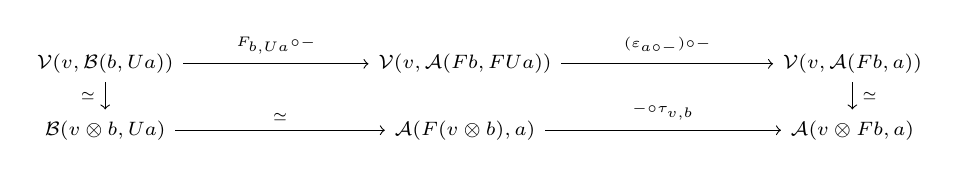
\begin{tikzpicture}[x=1.0em,y=1.5em,every node/.style={font=\scriptsize}]
  \node (TL) at (0,1.6) {$\mathcal{V}(v,\mathcal{B}(b,Ua))$};
  \node (TM) at (13.0,1.6) {$\mathcal{V}(v,\mathcal{A}(Fb,FUa))$};
  \node (TR) at (27.0,1.6) {$\mathcal{V}(v,\mathcal{A}(Fb,a))$};
  \node (BL) at (0,0) {$\mathcal{B}(v\otimes b,Ua)$};
  \node (BM) at (13.0,0) {$\mathcal{A}(F(v\otimes b),a)$};
  \node (BR) at (27.0,0) {$\mathcal{A}(v\otimes Fb,a)$};
  \draw[->] (TL) -- node[above]{$\scriptstyle F_{b,Ua}\circ-$} (TM);
  \draw[->] (TM) -- node[above]{$\scriptstyle(\varepsilon_{a\circ-})\circ-$} (TR);
  \draw[->] (0,1.15) -- node[left]{$\scriptstyle\simeq$} (0,0.5);
  \draw[->] (27.0,1.15) -- node[right]{$\scriptstyle\simeq$} (27.0,0.5);
  \draw[->] (BL) -- node[above]{$\scriptstyle\simeq$} (BM);
  \draw[->] (BM) -- node[above]{$\scriptstyle-\circ\tau_{v,b}$} (BR);
\end{tikzpicture}
\end{center}
其中那三个\trIsomorphism{}由跨越非富集\trAdjunction{}作转置而定义。由于这是
一个由集合之间的函数构成的图表，为验证其交换性，只需考虑一个\trElement{}
$f\colon v\to\mathcal{B}(b,Ua)$；其在两个复合之下的像是复合映射
\[ v\otimes Fb\xrightarrow{\ f\otimes Fb\ }\mathcal{B}(b,Ua)\otimes Fb
   \xrightarrow{\ F_{b,Ua}\otimes Fb\ }\mathcal{A}(Fb,FUa)\otimes Fb
   \xrightarrow{\ \mathrm{ev}\ }FUa\xrightarrow{\ \varepsilon_{a}\ }a \]
它居于 $\mathcal{A}$ 的底范畴之中。由于 $F$ 保持张量，映射 $\tau_{v,b}$ 是一个%
\trIsomorphism，于是由非富集\trYonedaLemma，\eqref{eq:adjunction-composite}
也是一个\trIsomorphism。
\end{proof}

\subsection*{练习}

\begin{exercise}\label{ex:enriched-left-adjoints-preserve-tensors}
证明：富集左伴随保持张量，并且定义非富集左伴随。
\end{exercise}

\begin{exercise}\label{ex:tensored-diagram-category}
设 $\mathcal{J}$ 是一个小的非富集\trCategory{}并设 $\mathcal{C}$ 是一个
$\mathcal{V}$-范畴。证明：若 $\mathcal{C}$ 是张量化的或余张量化的，则
$\mathcal{C}^{\mathcal{J}}$ 亦然。
\end{exercise}

   %

\providecommand{\sSet}{s\mathcal{S}et}
\providecommand{\colim}{\operatorname{colim}}

\section{锥形极限与余极限}\label{sec:conical-limits-and-colimits}

试考虑一支图表 $F\colon\mathcal{J}\to\mathcal{C}$，其由一个 1-\trCategory{}
$\mathcal{J}$ 标引，而取值于一个 $\mathcal{V}$-\trCategory{} $\mathcal{C}$。
图表 $F$ 之上带峰顶 $\ell\in\mathcal{C}$ 的一支\trCone{} $\lambda$ 是一支极限
锥，若与 $\lambda$ 的复合诱导诸 hom-集之间的一个双射
\[ \mathcal{C}(x,\ell)_{0}\xrightarrow[\ \simeq\ ]{\ \lambda\circ-\ }
   \lim_{j\in\mathcal{J}}\mathcal{C}(x,Fj)_{0} \]
对一切 $x\in\mathcal{C}$。若 $\mathcal{V}$ 容许形状为 $\mathcal{J}$ 的%
\trLimit，则该复合映射提升入 $\mathcal{V}$ 中，并且，断言极限锥之通常%
\trUniversalProperty{}的一个更强版本乃是自然之事：要求与 $\lambda$ 的复合诱导
诸 $\mathcal{V}$-对象之间的一个\trIsomorphism，而不只是诸 hom-集之间的一个。
这就给出了取值于一个\trEnrichedCategory{}的图表之\emph{锥形极限}的概念。%
\emph{锥形余极限}对偶地定义（见\cref{def:conical-limit-colimit}）。

底集函子 $(-)_{0}\coloneqq\mathcal{V}(1,-)\colon\mathcal{V}\to\mathcal{S}et$
保持\trLimit，并把 $\mathcal{V}$ 中的\trIsomorphism{}带为诸集合之间的双射。
于是，锥形极限必然定义 1-范畴的\trLimit，故我们特别关注：要把一个 1-范畴的%
\trLimit{}富集成一个锥形极限，究竟需要些什么。沿这条路线的第一个观察是：取值
于\trCartesianClosed{}\trCategory{} $\mathcal{V}$ 的图表之\trLimit{}与%
\trColimit{}总是富集而定义锥形极限与锥形余极限。

\begin{lemma}\label{lem:cc-conical}
若 $\mathcal{V}$ 是一个\trCartesianClosed{}\trCategory，则图表
$F\colon\mathcal{J}\to\mathcal{V}$ 之上的任一 1-范畴的极限锥
$\lambda\colon\Delta\lim F\Rightarrow F$，或其之下的任一 1-范畴的余极限锥
$\gamma\colon F\Rightarrow\Delta\colim F$，都产生诸\trIsomorphism
\[ (\lim F)^{v}\cong\lim_{j\in\mathcal{J}}(Fj)^{v}
   \qquad\text{以及}\qquad
   v^{\colim F}\cong\lim_{j\in\mathcal{J}^{\mathrm{op}}}v^{Fj} \]
其居于 $\mathcal{V}$ 之中，且在 $v\in\mathcal{V}$ 中是 $\mathcal{V}$-自然的。
\end{lemma}

\begin{proof}
对任何 $v\in\mathcal{V}$，指数\trFunctor{}
$(-)^{v}\colon\mathcal{V}\to\mathcal{V}$ 是乘积\trFunctor{}
$-\times v\colon\mathcal{V}\to\mathcal{V}$ 的\trRightAdjoint；正因如此，它保持%
\trLimit，这就产生了陈述中的第一个\trIsomorphism；而
$v^{-}\colon\mathcal{V}^{\mathrm{op}}\to\mathcal{V}$ 作为互为右伴随者，则把%
\trColimit{}带为\trLimit，这就建立了第二个。
\end{proof}

从本节余下部分起，设 $\mathcal{V}$ 是一个\trComplete{}\trCartesianClosed{}%
\trCategory，从而编码锥形极限与锥形余极限之\trUniversalProperty{}的那些
$\mathcal{V}$ 中的\trLimit{}被设定为存在。

\begin{definition}\label{def:conical-limit-colimit}
设 $\mathcal{C}$ 是一个 $\mathcal{V}$-\trCategory{}并设 $\mathcal{J}$ 是一个
小 1-\trCategory。非富集图表 $F\colon\mathcal{J}\to\mathcal{C}$ 的%
\textbf{锥形极限}（conical limit）由一个对象 $\ell\in\mathcal{C}$ 与一支%
\trCone{} $\lambda\colon\Delta\ell\Rightarrow F$ 给出，后者诱导诸 hom-对象
之间的一个 $\mathcal{V}$-自然\footnote{对任何\trCone{}
$\lambda\colon\Delta\ell\Rightarrow F$——不必是极限锥——复合定义一个映射
$\lambda\circ-\colon\mathcal{C}(x,\ell)\to\lim\limits_{j\in\mathcal{J}}\mathcal{C}(x,Fj)$，
其在 $x$ 中是 $\mathcal{V}$-自然的（见\cref{ex:conical-map-vnatural}）。其证
由与\cref{exa:post-composition-vnatural-transformation}中所用者本质相同的论证
给出——该论证证明：富集范畴之底范畴中的诸箭头在诸可表示函子之间诱导富集%
\trNaturalTransformation。于是，刻画锥形极限的那个\trUniversalProperty{}之
内容即在于：这个 $\mathcal{V}$-自然映射是\trInvertible。}\trIsomorphism
\[ \mathcal{C}(x,\ell)\xrightarrow[\ \simeq\ ]{\ \lambda\circ-\ }
   \lim_{j\in\mathcal{J}}\mathcal{C}(x,Fj)
   \qquad\in\ \mathcal{V} \]
对一切 $x\in\mathcal{C}$。对偶地，\textbf{锥形余极限}（conical colimit）由一
个对象 $c\in\mathcal{C}$ 与一支\trCone{} $\gamma\colon F\Rightarrow\Delta c$
给出，后者诱导一个 $\mathcal{V}$-自然\trIsomorphism
\[ \mathcal{C}(c,x)\xrightarrow[\ \simeq\ ]{\ \gamma^{*}\ }
   \lim_{j\in\mathcal{J}^{\mathrm{op}}}\mathcal{C}(Fj,x)
   \qquad\in\ \mathcal{V} \]
对一切 $x\in\mathcal{C}$。
\end{definition}

刻画锥形极限与锥形余极限的那些\trIsomorphism，与刻画 1-范畴的\trLimit{}和%
\trColimit{}的那些通常\trIsomorphism{}极为相似，只是有一个非常重要的差别：它
们设定的是 $\mathcal{V}$ 中的\trIsomorphism，而非 $\mathcal{S}et$ 中的%
\trIsomorphism。在 $\mathcal{V}=\sSet$ 的情形，这个单纯集之间的%
\trIsomorphism{}所底下的那个顶点之间的\trIsomorphism{}描述的正是通常的
1-范畴\trUniversalProperty。称一个\trLimit{}是\emph{锥形的}而不只是%
\emph{1-范畴的}，即是断言这个\trUniversalProperty{}延伸到一切正维数。

检视\cref{def:conical-limit-colimit}，我们立即看到：

\begin{proposition}\label{prop:conical-representables}
一支 1-范畴的极限锥是锥形的，恰当时它被一切取值于 $\mathcal{V}$ 中的可表示
函子 $\mathcal{C}(x,-)\colon\mathcal{C}\to\mathcal{V}$ 所保持；而一支 1-范畴
的余极限锥是锥形的，恰当时它被一切取值于 $\mathcal{V}$ 中的可表示函子
$\mathcal{C}(-,x)\colon\mathcal{C}^{\mathrm{op}}\to\mathcal{V}$ 所保持。
\end{proposition}

\cref{lem:cc-conical}之证明可加以推广以证：

\begin{proposition}\label{prop:tensors-cotensors-conical}
在一个张量化的富集范畴 $\mathcal{C}$ 中，一切 1-范畴的\trLimit{}都是锥形的；
而在一个余张量化的富集范畴 $\mathcal{C}$ 中，一切 1-范畴的\trColimit{}都是
锥形的。
\end{proposition}

\begin{proof}
由\cref{prop:conical-representables}，为证 $\mathcal{V}$-\trCategory{}
$\mathcal{C}$ 中的一个 1-范畴的\trLimit{}是锥形的，只需证明它被诸取值于
$\mathcal{V}$ 中的可表示函子 $\mathcal{C}(x,-)\colon\mathcal{C}\to\mathcal{V}$
对一切 $x\in\mathcal{C}$ 所保持。若 $\mathcal{C}$ 容许张量，则这些\trFunctor{}%
中的每一个都容有一个\trLeftAdjoint；作为\trRightAdjoint，后者必然保持陈述中
的那些 1-范畴的\trLimit。
\end{proof}

与\cref{prop:conical-representables}相类比，我们有：

\begin{proposition}\label{prop:cotensor-preservation}
设 $\mathcal{C}$ 在 $\mathcal{V}$ 上富集且余张量化。非富集图表
$F\colon\mathcal{J}\to\mathcal{C}$ 的一个\trLimit{}是一个锥形极限，当且仅当
它被与一切对象 $v\in\mathcal{V}$ 的余张量所保持。
\end{proposition}

\begin{proof}
余张量是 $\mathcal{V}$-富集的\trRightAdjoint，后者保持锥形极限。其实质在于：
被余张量保持即足以把一个 1-范畴的\trLimit{}富集为一个 $\mathcal{V}$-范畴的%
\trLimit。

由\cref{prop:conical-representables}，一支 1-范畴的极限锥
$\lambda\colon\Delta\ell\Rightarrow F$ 是锥形的，恰当时它被一切取值于
$\mathcal{V}$ 中的可表示函子 $\mathcal{C}(x,-)\colon\mathcal{C}\to\mathcal{V}$
所保持。为见自然映射
\[ \mathcal{C}(x,\ell)\xrightarrow{\ \lambda\circ-\ }
   \lim_{j\in\mathcal{J}}\mathcal{C}(x,Fj) \]
是 $\mathcal{V}$ 中的一个\trIsomorphism，我们诉诸非富集的\trYonedaLemma{}并
论证：对任何 $v\in\mathcal{V}$，在施加非富集可表示函子
$\mathcal{V}(v,-)\colon\mathcal{V}\to\mathcal{S}et$ 时，这个映射诱导一个%
\trIsomorphism。为见这一可逆性，注意到诱导出的 hom-集之间的映射恰好居于如下
交换图表之中
\begin{center}
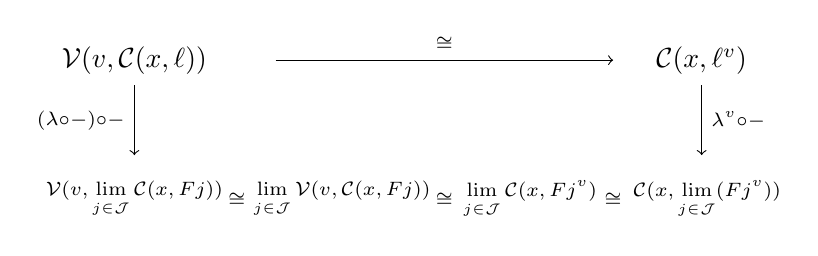
\begin{tikzpicture}[x=1em,y=1.4em]
  \node (tl) at (0,2.2) {$\mathcal{V}(v,\mathcal{C}(x,\ell))$};
  \node (tr) at (20.5,2.2) {$\mathcal{C}(x,\ell^{v})$};
  \draw[->] (5.1,2.2) -- node[above]{$\scriptstyle\cong$} (17.3,2.2);
  \draw[->] (0,1.55) -- node[left]{$\scriptstyle(\lambda\circ-)\circ-$} (0,-0.25);
  \draw[->] (20.5,1.55) -- node[right]{$\scriptstyle\lambda^{v}\circ-$} (20.5,-0.25);
  \node[font=\scriptsize] (b1) at (0,-1.4)
    {$\mathcal{V}(v,\displaystyle\lim_{j\in\mathcal{J}}\mathcal{C}(x,Fj))$};
  \node[font=\scriptsize] at (3.7,-1.4) {$\cong$};
  \node[font=\scriptsize] (b2) at (7.5,-1.4)
    {$\displaystyle\lim_{j\in\mathcal{J}}\mathcal{V}(v,\mathcal{C}(x,Fj))$};
  \node[font=\scriptsize] at (11.2,-1.4) {$\cong$};
  \node[font=\scriptsize] (b3) at (14.3,-1.4)
    {$\displaystyle\lim_{j\in\mathcal{J}}\mathcal{C}(x,Fj^{v})$};
  \node[font=\scriptsize] at (17.3,-1.4) {$\cong$};
  \node[font=\scriptsize] (b4) at (20.7,-1.4)
    {$\mathcal{C}(x,\displaystyle\lim_{j\in\mathcal{J}}(Fj^{v}))$};
\end{tikzpicture}
\end{center}
其中诸水平\trIsomorphism{}表达余张量的非富集\trUniversalProperty，以及非富集
可表示函子保持\trLimit{}这一事实。

说诸余张量保持\trLimit{} $\ell\cong\lim\limits_{j\in\mathcal{J}}Fj$，即意指
$\ell^{v}\cong(\lim\limits_{j\in\mathcal{J}}Fj)^{v}\cong\lim\limits_{j\in\mathcal{J}}(Fj)^{v}$；
故由\trYonedaLemma，右竖直的映射是一个\trIsomorphism，从而左竖直的映射亦然。
\end{proof}

\subsection*{练习}

\begin{exercise}\label{ex:conical-map-vnatural}
试考虑一支图表 $F\colon\mathcal{J}\to\mathcal{C}$——其由一个 1-\trCategory{}%
标引而取值于一个 $\mathcal{V}$-\trCategory——以及一支\trCone{}
$\lambda\colon\Delta\ell\Rightarrow F$。假设 $\mathcal{V}$ 容有形状为
$\mathcal{J}$ 的\trLimit，试定义一个典范映射
$\lambda\circ-\colon\mathcal{C}(x,\ell)\to\lim\limits_{j\in\mathcal{J}}\mathcal{C}(x,Fj)$，
并沿\cref{exa:post-composition-vnatural-transformation}的路线论证：它是
$\mathcal{V}$-自然的。
\end{exercise}

\begin{exercise}[{\cite[第~306~页]{bib67}}]\label{ex:2cat-tensors-conical}
将\cref{prop:tensors-cotensors-conical}之结果特殊化，以证明下述结论：在任何
一个容许与\trWalkingArrow{}范畴 $2$ 取张量的 2-\trCategory{} $\mathcal{C}$
中，$\mathcal{C}$ 所容有的任何 1-范畴的\trLimit{}都自动是锥形的。%
\footnote{本陈述断言：与 $2$ 取张量之存在，蕴涵 1 维\trLimit{}的%
\trUniversalProperty{}自动带有一个额外的 2 维面向，如围绕第 1 章中的%
\cref{prop:cartesian-closure}的讨论所例示的那样。}
\end{exercise}

   %

\providecommand{\Cat}{\mathcal{C}at}
\providecommand{\sSet}{s\mathcal{S}et}
\providecommand{\wlim}{\operatorname{lim}}
\providecommand{\wcolim}{\operatorname{colim}}
\providecommand{\lan}{\operatorname{lan}}
\providecommand{\ran}{\operatorname{ran}}
\providecommand{\Fun}{\operatorname{Fun}}
\providecommand{\qcor}[1]{\ulcorner#1\urcorner}   %

\section{\trWeightedLimit{}与\trWeightedColimit}\label{sec:weighted-limits-and-colimits}

A.4 节的余张量与 A.5 节的锥形极限，皆为我们如今引入的更为一般的%
\emph{\trWeightedLimit}概念的实例。我们继续在\trComplete{}且\trCocomplete{}的%
\trCartesianClosed{}\trCategory{} $(\mathcal{V},\times,1)$ 的语境中工作。我们
心目中的例子是 $(\sSet,\times,1)$、其\trCartesianClosed{}子范畴
$(\Cat,\times,1)$，或者再往下一层的\trCartesianClosed{}子范畴
$(\mathcal{S}et,\times,1)$。

通常的\trLimit{}与\trColimit{}是那样一些对象：它们表示「以一个给定峰顶居于
一个固定\trDiagram{}之上或居于其下」的诸锥所构成的\trFunctor。\trWeightedLimit%
{}与\trWeightedColimit{}以类似的方式定义，不同之处只在于：居于一个\trDiagram%
{}之上或之下的诸锥可以带有\trExotic{}「形状」，而且这些形状容许随加标于该%
\trDiagram{}的那些对象而变化。更正式地，在 $\mathcal{V}$-富集的语境中，%
\emph{权}（weight）——它定义居于一个由 $\mathcal{A}$ 加标的\trDiagram{}之上、
或居于一个由 $\mathcal{A}^{\mathrm{op}}$ 加标的\trDiagram{}之下的锥之「形状」
——取 $\mathcal{V}^{\mathcal{A}}$ 中一个\trFunctor{}的形式；注意加标范畴
$\mathcal{A}$ 可以是 $\mathcal{V}$-富集的，这与 A.5 节所考虑的诸\trDiagram%
{}不同。

我们将从三种不同的视角发展\trWeightedLimit{}与\trWeightedColimit{}的一般概念，
并按与逻辑顺序相反的次序引入这三者，因为我们发现这条路线最为直观。我们首先
描述——当它们存在时——刻画\trWeightedLimit{}与\trWeightedColimit{}二函子的
那些公理。继而解释：在假定某些其他\trLimit{}与\trColimit{}存在的条件下，
\trWeightedLimit{}与\trWeightedColimit{}可以如何被构造出来。最后我们引入定义
一个特定的\trWeightedLimit{}或\trWeightedColimit{}的一般\trUniversalProperty，
它确切地规定了刚刚引入的那些概念要真正存在所需的一切。

\begin{definition}[\trWeightedLimit{}与余极限，公理式的]\label{def:weighted-limit-colimit-axiomatic}
对一个小的 $\mathcal{V}$-范畴 $\mathcal{A}$ 与一个大的 $\mathcal{V}$-范畴
$\mathcal{C}$，\textbf{\trWeightedLimit}与\textbf{\trWeightedColimit{}二函子}
\[ \wlim_{-}\colon(\mathcal{V}^{\mathcal{A}})^{\mathrm{op}}\times
     \mathcal{C}^{\mathcal{A}}\to\mathcal{C}
   \qquad\text{以及}\qquad
   \wcolim_{--}\colon\mathcal{V}^{\mathcal{A}}\times
     \mathcal{C}^{\mathcal{A}^{\mathrm{op}}}\to\mathcal{C} \]
在它们存在之时，由下述一对公理刻画：
\begin{itemize}
\item 带可表示之权的加权余／极限在表示对象处求值：
\[ \wlim_{\mathcal{A}(a,-)}F\cong Fa
   \qquad\text{以及}\qquad
   \wcolim_{\mathcal{A}(-,a)}G\cong Ga. \]
\item 加权余／极限二函子在权上是余连续的：对任何\trDiagram{}
  $F\in\mathcal{C}^{\mathcal{A}}$ 与 $G\in\mathcal{C}^{\mathcal{A}^{\mathrm{op}}}$，
  \trFunctor{} $\wcolim_{-}G$ 保持\trColimit，而\trFunctor{} $\wlim_{-}F$ 把%
  \trColimit{}带为\trLimit。\footnote{更精确地说，正如%
  \cref{prop:weighted-limit-definitions-agree}所证明的，\trWeightedColimit%
  {}\trFunctor{} $\wcolim_{-}G$ 保持\trWeightedColimit，而%
  \trWeightedLimit{}\trFunctor{}
  $\wlim_{-}F$ 把\trWeightedColimit{}带为\trWeightedLimit。}
\end{itemize}
\end{definition}

我们把公理 (ii) 诠释为：权可以「按需定制」（made-to-order）——一个作为诸%
可表示\trFunctor{}的\trColimit{}而构造出的权——一切取值于 $\mathcal{V}$ 中的%
\trFunctor{}皆属此类——将会规定所期望的\trUniversalProperty。

\begin{definition}[\trWeightedLimit{}与余极限，构造式的]\label{def:weighted-limit-colimit-constructive}
以 $W\in\mathcal{V}^{\mathcal{A}}$ \textbf{加权}（weighted by）的\trDiagram{}
$F\in\mathcal{C}^{\mathcal{A}}$ 之\textbf{\trLimit}由函子余张量积（functor
cotensor product）计算：
\begin{rveq}\label{eq:functor-cotensor-product}
\wlim_{W}F\coloneqq\int\limits_{a\in\mathcal{A}}Fa^{Wa}
  \coloneqq\mathrm{eq}\left(\;
    \prod_{a\in\mathcal{A}}Fa^{Wa}
    \Longrightarrow
    \prod_{a,b\in\mathcal{A}}Fb^{\mathcal{A}(a,b)\times Wa}\;\right),
\end{rveq}
其中的乘积与等化子应按 A.5 节中的\cref{def:conical-limit-colimit}之意义诠释为锥形极限。等化子%
图表中的诸映射由 hom-对象 $\mathcal{A}(a,b)$ 在 $\mathcal{V}$-函子 $W$ 与 $F$
上的作用 $\mathcal{A}(a,b)\times Wa\to Wb$ 与 $Fa\to Fb^{\mathcal{A}(a,b)}$
诱导而出。
对偶地，以 $W\in\mathcal{V}^{\mathcal{A}}$ 加权的\trDiagram{}
$G\in\mathcal{C}^{\mathcal{A}^{\mathrm{op}}}$ 之\textbf{\trColimit}由函子张量积
（functor tensor product）计算：
\begin{rveq}\label{eq:functor-tensor-product}
\wcolim_{W}G\coloneqq\int\limits^{a\in\mathcal{A}}Wa\otimes Ga
  \coloneqq\mathrm{coeq}\left(\;
    \coprod_{a,b\in\mathcal{A}}\bigl(Wa\times\mathcal{A}(a,b)\bigr)\otimes Gb
    \Longrightarrow
    \coprod_{a\in\mathcal{A}}Wa\otimes Ga\;\right),
\end{rveq}
其中的余积与余等化子应诠释为锥形余极限。余等化子图表中的两支映射，一支由
$\mathcal{A}(a,b)$ 在反变 $\mathcal{V}$-函子 $G$ 上的作用
$\mathcal{A}(a,b)\otimes Gb\to Ga$ 诱导而出，另一支则一如前述地使用
$\mathcal{A}(a,b)$ 在 $W$ 上的协变作用。
\end{definition}

\begin{definition}[\trWeightedLimit{}与余极限，泛性质]\label{def:weighted-limit-colimit-universal-property}
\trDiagram{} $F\in\mathcal{C}^{\mathcal{A}}$ 以 $W\in\mathcal{V}^{\mathcal{A}}$
加权的\textbf{\trLimit} $\wlim_{W}F$ 与\trDiagram{}
$G\in\mathcal{C}^{\mathcal{A}^{\mathrm{op}}}$ 以 $W\in\mathcal{V}^{\mathcal{A}}$
加权的\textbf{\trColimit} $\wcolim_{W}G$ 由下述\trUniversalProperty{}刻画：
\begin{rveq}\label{eq:weighted-universal-property}
\mathcal{C}\bigl(x,\wlim_{W}F\bigr)\cong\mathcal{V}^{\mathcal{A}}\bigl(W,\mathcal{C}(x,F)\bigr)
\qquad\text{以及}\qquad
\mathcal{C}\bigl(\wcolim_{W}G,x\bigr)\cong\mathcal{V}^{\mathcal{A}}\bigl(W,\mathcal{C}(G,x)\bigr),
\end{rveq}
其中每一者都定义 $\mathcal{V}$ 中诸对象之间的一个\trIsomorphism，后者在 $x$ 上
是 $\mathcal{V}$-自然的。
\end{definition}

当加标范畴从上下文来看不明确时，我们可以在\trWeightedLimit{}与\trWeightedColimit{}的记号上添加
一个上标以指明它。\cref{prop:weighted-limit-definitions-agree}表明：这三个定义
刻画的是同样的对象。在证明它的途中，我们会得到一些因其自身之故而值得关切的
结果，并将它们单独记录如下。

\begin{lemma}\label{lem:complete-v-admits-weighted-limits}
一个\trComplete{}\trCartesianClosed{}\trCategory{} $\mathcal{V}$ 容有一切%
\trWeightedLimit——即由 \eqref{eq:functor-cotensor-product} 之公式所定义、满足
\eqref{eq:weighted-universal-property} 之自然\trIsomorphism{}与%
\cref{def:weighted-limit-colimit-axiomatic}之公理的\trWeightedLimit。显式地，对一个权
$W\colon\mathcal{A}\to\mathcal{V}$ 与一个\trDiagram{}
$F\colon\mathcal{A}\to\mathcal{V}$，\trWeightedLimit
\[ \wlim_{W}F\coloneqq\mathcal{V}^{\mathcal{A}}(W,F) \]
就是从 $W$ 到 $F$ 的诸 $\mathcal{V}$-\trNaturalTransformation{}的
$\mathcal{V}$-对象。\footnote{原书此处印作「from $W$ to $V$」；按上方显式公式
$\wlim_{W}F\coloneqq\mathcal{V}^{\mathcal{A}}(W,F)$，疑为「from $W$ to $F$」
之误，此处径改。——译者注}
\end{lemma}

\begin{proof}
由\trTerminal{}对象所表示的 $\mathcal{V}$-函子
$\mathcal{V}(1,-)\colon\mathcal{V}\to\mathcal{V}$ 自然同构于恒等\trFunctor。
于是，在\trDiagram{} $F\in\mathcal{V}^{\mathcal{A}}$ 取值于 $\mathcal{V}$-范畴
$\mathcal{V}$ 之中的情形下，于 \eqref{eq:weighted-universal-property} 的%
\trUniversalProperty{}中取 $x=1$，便有
\[ \wlim_{W}F\cong\mathcal{V}^{\mathcal{A}}(W,F). \]
与此同时，公式 \eqref{eq:functor-cotensor-product} 计算了%
\cref{def:vobject-natural-transformations}所引入的、从 $W$ 到 $F$ 的诸
$\mathcal{V}$-\trNaturalTransformation{}的 $\mathcal{V}$-对象
$\mathcal{V}^{\mathcal{A}}(W,F)$。\cref{thm:enriched-yoneda}的富集%
\trYonedaLemma{}证得第一条公理，而第二条公理可由
\eqref{eq:weighted-universal-property} 的\trUniversalProperty{}推出。
\end{proof}

诸 $\mathcal{V}$-\trNaturalTransformation{}的 $\mathcal{V}$-对象满足自然%
\trIsomorphism
\[ \mathcal{V}\bigl(v,\mathcal{V}^{\mathcal{A}}(W,F)\bigr)
   \cong\mathcal{V}^{\mathcal{A}}\bigl(W,\mathcal{V}(v,F)\bigr) \]
对任何 $v\in\mathcal{V}$。把「取值于 $\mathcal{V}$ 的诸\trFunctor{}的
$W$-\trWeightedLimit{}是诸\trNaturalTransformation{}的 $\mathcal{V}$-对象」这一观察应用
于诸\trFunctor{} $\mathcal{C}(x,F-)$ 与 $\mathcal{C}(G-,x)$，我们便可把自然%
\trIsomorphism{} \eqref{eq:weighted-universal-property} 重新表达为：

\begin{corollary}\label{cor:weighted-limits-representably-defined}
\eqref{eq:weighted-universal-property} 的\trWeightedLimit{}与\trWeightedColimit，作为 $\mathcal{V}$
中的\trWeightedLimit{}被可表示地定义：对 $W\in\mathcal{V}^{\mathcal{A}}$、
$F\in\mathcal{C}^{\mathcal{A}}$ 与 $G\in\mathcal{C}^{\mathcal{A}^{\mathrm{op}}}$，
\trWeightedLimit{}与\trWeightedColimit{}由在 $x$ 中 $\mathcal{V}$-自然的诸\trIsomorphism{}刻画：
\begin{rveq}\label{eq:weighted-representable-expression}
\mathcal{C}\bigl(x,\wlim_{W}F\bigr)\cong\wlim_{W}\mathcal{C}(x,F)
\qquad\text{以及}\qquad
\mathcal{C}\bigl(\wcolim_{W}G,x\bigr)\cong\wlim_{W}\mathcal{C}(G,x)
\end{rveq}
\end{corollary}

我们如今统一定义 A.6.1、定义 A.6.2 与定义 A.6.5 这三者。

\begin{proposition}\label{prop:weighted-limit-definitions-agree}
当 \eqref{eq:functor-cotensor-product} 与 \eqref{eq:functor-tensor-product} 的%
\trLimit{}与\trColimit{}存在时，它们所定义的对象满足\trUniversalProperty{}
\eqref{eq:weighted-universal-property}，或者等价地，满足
\eqref{eq:weighted-representable-expression}。由这些\trUniversalProperty{}所
定义的 $\mathcal{V}$-二函子满足\cref{def:weighted-limit-colimit-axiomatic}的
公理。
\end{proposition}

\begin{proof}
定义 A.6.2 与定义 A.6.5 之等价性——对\trWeightedLimit{}或\trWeightedColimit{}任一者而言——是
这一蕴含关系在取值于 $\mathcal{C}=\mathcal{V}$ 的\trWeightedLimit{}上的特例的直接推论，
后者已作为\cref{lem:complete-v-admits-weighted-limits}与%
\cref{cor:weighted-limits-representably-defined}证得。\eqref{eq:functor-cotensor-product}
中对 $\mathcal{A}$ 加标的诸\trLimit，同样以可表示的方式经由 $\mathcal{V}$ 中
类似的\trLimit{}来定义。于是，由 \eqref{eq:functor-cotensor-product} 所定义的
那个对象表示定义\trWeightedLimit{} $\wlim_{W}F$ 的 $\mathcal{V}$-\trFunctor{}
$\wlim_{W}\mathcal{C}(-,F)$。

尚须证明：定义 A.6.2 与定义 A.6.5 的\trWeightedLimit{}满足%
\cref{def:weighted-limit-colimit-axiomatic}的公理。在取值于 $\mathcal{V}$ 的%
\trDiagram{} $F\in\mathcal{V}^{\mathcal{A}}$ 的情形，公理 (i) 就是
$\mathcal{V}$-\trYonedaLemma：$\mathcal{V}^{\mathcal{A}}(\mathcal{A}(a,-),F)\cong Fa$，
已作为\cref{thm:enriched-yoneda}证得。再一次地，$F\in\mathcal{C}^{\mathcal{A}}$
的一般情形由取值于 $\mathcal{V}$ 的\trDiagram{}这一特例得出。为在 $\mathcal{C}$
中展示一个\trIsomorphism{} $\wlim_{\mathcal{A}(a,-)}F\cong Fa$，只需对一切
$x\in\mathcal{C}$ 在 $\mathcal{V}$ 中造出一个\trIsomorphism{}
$\mathcal{C}(x,\wlim_{\mathcal{A}(a,-)}F)\cong\mathcal{C}(x,Fa)$；而对%
\trFunctor{} $\mathcal{C}(x,F-)\in\mathcal{V}^{\mathcal{A}}$ 应用
\eqref{eq:weighted-representable-expression} 与刚才作出的那个观察，我们便拥有
这样一个自然\trIsomorphism。

至于公理 (ii)，考虑一个由权构成的\trDiagram{}
$W\colon\mathcal{J}^{\mathrm{op}}\to\mathcal{V}^{\mathcal{A}}$ 与一个
权 $V\in\mathcal{V}^{\mathcal{J}}$，使得 $\wcolim^{\mathcal{J}}_{V}W$ 是
$\mathcal{V}^{\mathcal{A}}$ 中的一个对象。对任何 $F\in\mathcal{C}^{\mathcal{A}}$，
我们将证明：$\mathcal{V}$-\trFunctor{}
$\wlim^{\mathcal{A}}_{-}F\colon(\mathcal{V}^{\mathcal{A}})^{\mathrm{op}}\to\mathcal{C}$
把诸权之\trDiagram{}的 $V$-\trWeightedColimit{}带到复合\trDiagram{}
$\wlim^{\mathcal{A}}_{W-}F\colon\mathcal{J}\to\mathcal{C}$ 的 $V$-\trWeightedLimit。

将\trUniversalProperty{} \eqref{eq:weighted-universal-property} 先施加于%
\trDiagram{} $F$ 与对象 $x$ 的 $\wcolim^{\mathcal{J}}_{V}W$-\trWeightedLimit、再施加于%
\trDiagram{} $W$ 与对象 $\mathcal{C}(x,F)$ 的 $V$-\trWeightedColimit，便给出诸%
\trIsomorphism：
\[ \mathcal{C}\bigl(x,\wlim^{\mathcal{A}}_{\wcolim^{\mathcal{J}}_{V}W}F\bigr)
   \cong\mathcal{V}^{\mathcal{A}}\bigl(\wcolim^{\mathcal{J}}_{V}W,\mathcal{C}(x,F)\bigr)
   \cong\mathcal{V}^{\mathcal{J}}\bigl(V,\mathcal{V}^{\mathcal{A}}\bigl(W,\mathcal{C}(x,F)\bigr)\bigr). \]
再把 \eqref{eq:weighted-universal-property} 施加两次——先施加于每个
$j\in\mathcal{J}$ 的权 $Wj$、再施加于权 $V$ 与\trDiagram{}
$\wlim^{\mathcal{A}}_{W-}F\colon\mathcal{J}\to\mathcal{C}$——我们便有
\[ \cong\mathcal{V}^{\mathcal{J}}\bigl(V,\mathcal{C}\bigl(x,\wlim^{\mathcal{A}}_{W-}F\bigr)\bigr)
   \cong\mathcal{C}\bigl(x,\wlim^{\mathcal{J}}_{V}\wlim^{\mathcal{A}}_{W-}F\bigr). \]
由\trYonedaLemma，这就证明了
\[ \wlim^{\mathcal{A}}_{\wcolim^{\mathcal{J}}_{V}W}F
   \cong\wlim^{\mathcal{J}}_{V}\wlim^{\mathcal{A}}_{W-}F, \]
亦即：\trWeightedLimit{}\trFunctor{} $\wlim^{\mathcal{A}}_{-}F$ 把诸权的一个%
\trWeightedColimit{}带到诸权的类似的\trWeightedLimit。
\end{proof}

\begin{remark}[对非富集的加标范畴]\label{rem:unenriched-indexing-categories}
当加标范畴非富集时，\cref{def:weighted-limit-colimit-constructive}中的极限与
余极限公式简化为
\begin{gather*}
\wlim_{W}F\cong\mathrm{eq}\left(\;
  \prod_{a\in\mathcal{A}}Fa^{Wa}
  \Longrightarrow
  \prod_{\mathcal{A}(a,b)}Fb^{Wa}\;\right)\\
\wcolim_{W}G\cong\mathrm{coeq}\left(\;
  \coprod_{\mathcal{A}(a,b)}Wa\otimes Gb
  \Longrightarrow
  \coprod_{a\in\mathcal{A}}Wa\otimes Ga\;\right)
\end{gather*}
而事实上，只需考虑非恒等箭头、甚至只需考虑原子箭头，便已足够。
\end{remark}

\begin{example}[锥形极限与余极限]\label{exa:conical-limits-colimits}
对任何小 $\mathcal{V}$-范畴 $\mathcal{A}$，取值于 $\mathcal{V}$ 的%
\trTerminal{}对象之上的\trConstantFunctor{}定义终权 $1\in\mathcal{V}^{\mathcal{A}}$。
分别对\trDiagram{} $F\in\mathcal{C}^{\mathcal{A}}$ 与
$G\in\mathcal{C}^{\mathcal{A}^{\mathrm{op}}}$，以这个权加权的诸\trLimit{}与诸%
\trColimit{}满足定义性\trUniversalProperty
\begin{gather*}
\mathcal{C}(x,\wlim_{1}F)\cong\mathcal{V}^{\mathcal{A}}\bigl(1,\mathcal{C}(x,F)\bigr)
  \cong\wlim_{1}\mathcal{C}(x,F)\\
\mathcal{C}(\wcolim_{1}G,x)\cong\mathcal{V}^{\mathcal{A}}\bigl(1,\mathcal{C}(G,x)\bigr)
  \cong\wlim_{1}\mathcal{C}(G,x),
\end{gather*}
它们说明：$\wlim_{1}F$ 与 $\wcolim_{1}G$ 分别表示「居于 $F$ 之上或居于 $G$
之下的诸 $\mathcal{V}$-富集锥形锥」所构成的诸\trFunctor。

当 $\mathcal{A}$ 是一个非富集的\trCategory{}时，这就恢复了刻画 A.5 节中的%
\cref{def:conical-limit-colimit}的\textbf{锥形极限}（conical limits）与\textbf{锥形余极限}（conical
colimits）的那个\trUniversalProperty，于是我们把这两个术语的用法扩展为泛指以%
终权加权的那些一般\trLimit{}与\trColimit；对锥形极限与锥形余极限，常用简化%
记法 $\wlim F\coloneqq\wlim_{1}F$ 与 $\wcolim G\coloneqq\wcolim_{1}G$。这解释了
「锥形的」这一名称：在诸\trWeightedLimit{}之中，锥形极限是那些带有通常锥体形状者——在
底范畴中涉及一支从峰顶（summit）指向\trDiagram{}中每个对象的箭头。从而，锥形%
\trLimit{}与\trColimit{}作为其权为\trTerminal{}对象的\trWeightedLimit{}与%
\trWeightedColimit{}的特例而出现。
\end{example}

\begin{example}[张量与余张量]\label{exa:tensors-and-cotensors}
一个由终权范畴 $\mathbb{1}$ 加标、取值于一个 $\mathcal{V}$-富集范畴
$\mathcal{C}$ 中的\trDiagram{}不过是 $\mathcal{C}$ 中的一个对象 $c$。这类%
\trDiagram{}的权则不过由另一个对象 $v\in\mathcal{V}$ 给出。\trDiagram{} $c$ 的
$v$-\trWeightedLimit{}由刻画\textbf{余张量} $c^{v}$ 的那个\trUniversalProperty
\[ \mathcal{C}\bigl(x,\wlim^{\mathbb{1}}_{v}c\bigr)\cong\mathcal{C}(x,c)^{v} \]
所定义，而\trDiagram{} $c$ 的 $v$-\trWeightedColimit{}则由刻画\textbf{\trTensor}
$v\otimes c$ 的那个\trUniversalProperty
\[ \mathcal{C}\bigl(\wcolim^{\mathbb{1}}_{v}c,x\bigr)\cong\mathcal{C}(c,x)^{v} \]
所定义。从而，余张量与张量作为其加标范畴为终权范畴的\trWeightedLimit{}与%
\trWeightedColimit{}的特例而出现。
\end{example}

\begin{example}[逗号]\label{exa:commas}
一个\trInfinityCosmos{} $\mathcal{K}$ 特别地是一个富集于\trSimplicialSet{}之上
的\trCategory。\trCommaInfinityCategory{}是\trInfinityCosmos{} $\mathcal{K}$ 中
如下\trDiagram{} $2\to\mathcal{K}$ 的\trLimit——该\trDiagram{}由余跨度
\[ C\xrightarrow{\;g\;}A\xleftarrow{\;f\;}B \]
给出——以如下\trDiagram{} $2\to\sSet$ 加权，后者由余跨度
\[ \mathbb{1}\;\overset{\,1\,}{\hookrightarrow}\;2\;\overset{\,0\,}{\hookleftarrow}\;\mathbb{1} \]
给出。在\cref{rem:unenriched-indexing-categories}的简化之下，\trWeightedLimit{}的公式化
为下述平行映射对的等化子
\begin{center}
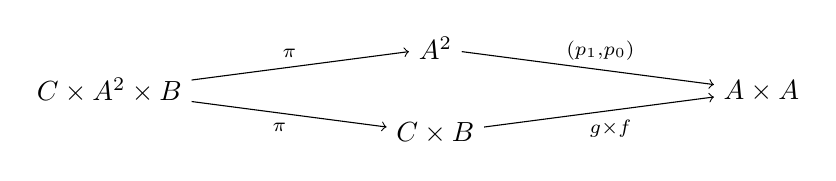
\begin{tikzpicture}[x=1.9em,y=1.4em]
  \node (L) at (0,0) {$C\times A^{2}\times B$};
  \node (T) at (6.2,1.1) {$A^{2}$};
  \node (B) at (6.2,-1.1) {$C\times B$};
  \node (R) at (12.4,0) {$A\times A$};
  \draw[->] (L) -- node[above,pos=0.45]{$\scriptstyle\pi$} (T);
  \draw[->] (L) -- node[below,pos=0.45]{$\scriptstyle\pi$} (B);
  \draw[->] (T) -- node[above,pos=0.55]{$\scriptstyle(p_{1},p_{0})$} (R);
  \draw[->] (B) -- node[below,pos=0.55]{$\scriptstyle g\times f$} (R);
\end{tikzpicture}
\end{center}
它计算 \eqref{eq:comma-pullback} 的拉回。\trUniversalProperty{} \eqref{eq:weighted-universal-property}
提供了 $\mathcal{K}$ 中的诸\trFunctor{} $\qcor{\alpha}\colon X\to\mathrm{Hom}_{A}(f,g)$
与诸单纯\trNaturalTransformation{}之间的一个对应，其
数据由恰好拼入两个交换方块的三支竖直虚映射给出：
\begin{center}
\begin{tikzpicture}[x=1.8em,y=1.4em]
  \node (1l) at (0,1.5) {$\mathbb{1}$};
  \node (two) at (3.6,1.5) {$2$};
  \node (1r) at (7.2,1.5) {$\mathbb{1}$};
  \draw[right hook->] (0.55,1.5) -- node[above]{$\scriptstyle 1$} (3.05,1.5);
  \draw[right hook->] (6.65,1.5) -- node[above]{$\scriptstyle 0$} (4.15,1.5);
  \draw[->,dashed] (0,1.05) -- node[left]{$\scriptstyle c$} (0,0.5);
  \draw[->,dashed] (3.6,1.05) -- node[right]{$\scriptstyle\qcor{\alpha}$} (3.6,0.5);
  \draw[->,dashed] (7.2,1.05) -- node[right]{$\scriptstyle b$} (7.2,0.5);
  \node (FL) at (0,0) {$\Fun(X,C)$};
  \node (FM) at (3.6,0) {$\Fun(X,A)$};
  \node (FR) at (7.2,0) {$\Fun(X,B)$};
  \draw[->] (1.35,0) -- node[below]{$\scriptstyle g\circ-$} (2.75,0);
  \draw[->] (6.35,0) -- node[below]{$\scriptstyle f\circ-$} (4.95,0);
\end{tikzpicture}
\end{center}
\end{example}

\begin{example}[作为加权余／极限的 Kan 扩张]\label{exa:kan-extensions-weighted}
计算一支非富集\trFunctor{} $F\colon C\to E$ 沿 $K\colon C\to D$ 的逐点左或右
Kan 扩张在对象 $d\in D$ 处之值的通常余极限或极限公式，可以由\trWeightedColimit{}或%
\trWeightedLimit{}简洁地表达为
\[ \lan_{K}F(d)\coloneqq\wcolim_{D(K-,d)}F
   \qquad\text{以及}\qquad
   \ran_{K}F(d)\coloneqq\wlim_{D(d,K-)}F. \]
\end{example}

\cref{def:weighted-limit-colimit-constructive}的诸公式给出了保证\trWeightedLimit{}或%
\trWeightedColimit{}得以存在的若干判据。

\begin{corollary}\label{cor:cotensors-conical-imply-weighted}
一个容有余张量、并对一切小的非富集\trDiagram{}形状容有锥形极限的 $\mathcal{V}$-%
\trCategory，便容有一切小的\trWeightedLimit。对偶地，一个容有张量、并对一切小的非富集%
\trDiagram{}形状容有锥形余极限的 $\mathcal{V}$-\trCategory，便容有一切小的%
\trWeightedColimit。
\end{corollary}

\begin{definition}\label{def:v-complete-v-cocomplete}
一个 $\mathcal{V}$-\trCategory{}是 $\mathcal{V}$-\textbf{\trComplete}
（$\mathcal{V}$-complete），若它容有诸小的 $\mathcal{V}$-\trWeightedLimit；或者等价
地，由\cref{cor:cotensors-conical-imply-weighted}，若它容有 $\mathcal{V}$ 中诸
对象所作的余张量以及小的锥形极限。对偶地，一个 $\mathcal{V}$-\trCategory{}是
$\mathcal{V}$-\textbf{\trCocomplete}（$\mathcal{V}$-cocomplete），若它容有诸
小的 $\mathcal{V}$-\trWeightedColimit；或者等价地，由%
\cref{cor:cotensors-conical-imply-weighted}，若它容有 $\mathcal{V}$ 中诸对象所
作的张量以及小的锥形余极限。
\end{definition}

\begin{remark}[论富集完备性的证明]\label{rem:proving-enriched-completeness}
在实践中，人们常如此证明一个 $\mathcal{V}$-\trCategory{}是完备的：证明其底%
\trCategory{}是完备的，并且该 $\mathcal{V}$-\trCategory{}同时容有余张量与张量
——后者乃是\trWeightedColimit{}的一个实例。然后施加\cref{prop:tensors-cotensors-conical}以确立：诸非富集的%
\trLimit{}事实上是锥形极限。
\end{remark}

我们以\trWeightedLimit{}与\trWeightedColimit{}一般理论中的若干结果来结束本节。从它们定义性的%
\trUniversalProperty{}出发立即可验证：

\begin{lemma}[受限\trDiagram{}的\trWeightedLimit]\label{lem:weighted-limits-restricted-diagrams}
设 $K\colon\mathcal{A}\to\mathcal{B}$ 是一支 $\mathcal{V}$-\trFunctor，
$W\colon\mathcal{A}\to\mathcal{V}$ 是一个权，而 $F\colon\mathcal{B}\to\mathcal{C}$
与 $G\colon\mathcal{B}^{\mathrm{op}}\to\mathcal{C}$ 是两个\trDiagram。于是，
受限\trDiagram{}的 $W$-\trWeightedLimit{}或\trWeightedColimit，同构于原\trDiagram{}的
$\lan_{K}W$-\trWeightedLimit{}或\trWeightedColimit：
\[ \wlim^{\mathcal{A}}_{W}(F\circ K)\cong\wlim^{\mathcal{B}}_{\lan_{K}W}F
   \qquad\text{以及}\qquad
   \wcolim^{\mathcal{A}}_{W}(G\circ K)\cong\wcolim^{\mathcal{B}}_{\lan_{K}W}G. \]
\end{lemma}

\begin{proof}
\cref{ex:prove-restricted-weighted-limits}。
\end{proof}

回忆\cref{def:vadjunction}：一个富集\trAdjunction{}由一对 $\mathcal{V}$-%
\trFunctor{} $F\colon\mathcal{B}\to\mathcal{A}$ 与
$U\colon\mathcal{A}\to\mathcal{B}$ 连同一族在两个变量中都是 $\mathcal{V}$-自然的%
\trIsomorphism{} $\mathcal{A}(Fb,a)\cong\mathcal{B}(b,Ua)$ 构成。通常的
Yoneda 式论证经富集化而表明：

\begin{proposition}\label{prop:enriched-adjoints-preserve-weighted-limits}
富集右伴随保持\trWeightedLimit，而富集左伴随保持\trWeightedColimit。
\end{proposition}

\begin{proof}
\cref{ex:prove-adjoints-preserve-weighted}。
\end{proof}

\subsection*{练习}

\begin{exercise}\label{ex:weighted-limits-of-simplicial-set}
把富集之基 $\mathcal{V}$ 取为 $\mathcal{S}et$，试计算单纯集 $X$——把它视作
$\mathcal{S}et^{\boldsymbol{\Delta}^{\mathrm{op}}}$ 中的一个\trDiagram{}——的
下列诸\trWeightedLimit，其权分别取：
\begin{enumerate}[label=(\roman*)]
\item 标准 $n$-\trSimplex{}
  $\Delta[n]\in\mathcal{S}et^{\boldsymbol{\Delta}^{\mathrm{op}}}$；
\item $n$-\trSimplex{}的\textbf{\trSpine}——把从 $i$ 到 $i+1$ 的那 $n$ 条边
  粘合为一条可复合的路径所得的 $\Delta[n]$ 的单纯子集；
\item $n$-\trSimplex{}边缘
  $\partial\Delta[n]\in\mathcal{S}et^{\boldsymbol{\Delta}^{\mathrm{op}}}$。
  \footnote{以 $\partial\Delta[n]$ 加权的单纯对象之\trLimit{}称为第 $n$ 个%
  \textbf{匹配对象}（$n$th-matching object）（见定义 C.4.14）。}
\end{enumerate}
\end{exercise}

\begin{exercise}\label{ex:prove-restricted-weighted-limits}
证明\cref{lem:weighted-limits-restricted-diagrams}。
\end{exercise}

\begin{exercise}\label{ex:prove-adjoints-preserve-weighted}
证明\cref{prop:enriched-adjoints-preserve-weighted-limits}。
\end{exercise}

\begin{exercise}\label{ex:enriched-profunctor-weights}
\begin{enumerate}[label=(\roman*)]
\item 把\trWeightedLimit{}与\trWeightedColimit{}的定义扩展到容许权 $W$ 为一个\textbf{富集泛函子}
  （enriched profunctor）——意即一支 $\mathcal{V}$-\trFunctor{}
  $W\colon\mathcal{B}^{\mathrm{op}}\times\mathcal{A}\to\mathcal{V}$，其中
  $\mathcal{A}$ 与 $\mathcal{B}$ 是小 $\mathcal{V}$-\trCategory{}——并使得%
  \trWeightedLimit{}与\trWeightedColimit{}\trFunctor{}具有如下形式：
  \[ (\mathcal{V}^{\mathcal{B}^{\mathrm{op}}\times\mathcal{A}})^{\mathrm{op}}
       \times\mathcal{C}^{\mathcal{A}}
       \xrightarrow{\ \wlim_{--}\ }\mathcal{C}^{\mathcal{B}}
     \qquad\text{以及}\qquad
     \mathcal{V}^{\mathcal{B}^{\mathrm{op}}\times\mathcal{A}}
       \times\mathcal{C}^{\mathcal{B}}
       \xrightarrow{\ \wcolim_{--}\ }\mathcal{C}^{\mathcal{A}} \]
\item 证明 (i) 中的\trWeightedLimit{}与\trWeightedColimit{}二函子构成一个双变量伴随的三分之二，
  其带有一个 $\mathcal{V}$-自然\trIsomorphism
\[ \mathcal{C}^{\mathcal{A}}\bigl(\wcolim_{W}G,F\bigr)
   \cong\mathcal{C}^{\mathcal{B}}\bigl(G,\wlim_{W}F\bigr) \]
  对 $W\in\mathcal{V}^{\mathcal{B}^{\mathrm{op}}\times\mathcal{A}}$、
  $F\in\mathcal{C}^{\mathcal{A}}$ 与 $G\in\mathcal{C}^{\mathcal{B}}$。
\item (ii) 的双变量伴随的第三个二函子是什么？
\end{enumerate}
\end{exercise}

   %

\providecommand{\Cat}{\mathcal{C}at}
\providecommand{\sSet}{s\mathcal{S}et}

\section{\trChangeOfBase}\label{sec:change-of-base}

「\trChangeOfBase」（change of base）最初由 Eilenberg 与 Kelly 在 \cite{bib41}
中考虑，指的是这样一种系统性的程序：把对一个范畴 $\mathcal{V}$ 的富集转换为对
另一个范畴 $\mathcal{W}$ 的富集。\cref{cor:vcat-two-category}指出：对一个%
\trCartesianClosed{}范畴 $\mathcal{V}$，存在一个由 $\mathcal{V}$-范畴、
$\mathcal{V}$-函子与 $\mathcal{V}$-自然变换组成的 2-\trCategory{}
$\mathcal{V}\text{-}\Cat$。第一个主要结果即\cref{prop:change-of-base-2-functor}，
它给出这样的条件：使一个介于\trCartesianClosed{}范畴之间的\trFunctor{}
$T\colon\mathcal{V}\to\mathcal{W}$ 诱导一个换基 2-\trFunctor{}
$T_{*}\colon\mathcal{V}\text{-}\Cat\to\mathcal{W}\text{-}\Cat$。

我们在此工作的语境不如 Eilenberg 与 Kelly 所考虑的那般一般——我们的基范畴是%
\trCartesianClosed{}，而他们的则是封闭对称幺半的——于是我们采取一条覆盖
我们全部例子且更易于解释的捷径。一般地，造出一个换基 2-函子所需要的，只是
对称幺半范畴之间的一个\emph{松幺半函子}（lax monoidal functor）；但我们在%
\trCartesianClosed{}范畴之间遇到的松幺半函子事实上都保持有限积，于是我们便
满足于把这一情形下的结果阐明出来。

回忆：介于\trCartesianClosed{}范畴之间的一个\trFunctor{}
$T\colon\mathcal{V}\to\mathcal{W}$ \textbf{保持有限积}（preserves finite
products），恰当对任何 $u$，$v\in\mathcal{V}$ 所定义的自然映射
\[ T(u\times v)\xRightarrow{\sim}Tu\times Tv
   \qquad\text{以及}\qquad
   T1\xRightarrow{\sim}1 \]
是\trIsomorphism。例如：

\begin{example}\label{exa:underlying-set-product-preserving}
由于可表示函子保持积，对任何\trCartesianClosed{}范畴 $\mathcal{V}$，底集函子
$(-)_{0}\colon\mathcal{V}\to\mathcal{S}et$ 是保持积的。
\end{example}

\begin{example}\label{exa:coproduct-functor-product-preserving}
在一个\trCartesianClosed{}范畴 $\mathcal{V}$ 中，有限积对任意\trCoproduct{}%
分配。特别地，对任何集合 $X$ 与 $Y$，在\trTerminal{}对象 $1$ 的诸%
\trCoproduct{}之间存在一个\trIsomorphism
\[ \coprod_{X\times Y}1\cong\bigl(\coprod_{X}1\bigr)\times
   \bigl(\coprod_{Y}1\bigr) \]
这就证明了\trFunctor
\[ \mathcal{S}et\xrightarrow{\ \coprod_{-}1\ }\mathcal{V} \]
是保持有限积的。
\end{example}

一个保持有限积的\trFunctor{}可以按下述方式用来更换基。

\begin{proposition}\label{prop:change-of-base-2-functor}
一个介于\trCartesianClosed{}范畴之间的、保持有限积的\trFunctor{}
$T\colon\mathcal{V}\to\mathcal{W}$ 诱导一个换基 2-\trFunctor
\[ \mathcal{V}\text{-}\Cat\xrightarrow{\ T_{*}\ }\mathcal{W}\text{-}\Cat. \]
\end{proposition}

沿这些路线的一个早期观察首先表述于 \cite[II.6.3]{bib41}，其证明留给读者。我们
采取同样的策略，把诸图表追索（diagram chase）留给读者或 \cite[4.2.4]{bib31}，
而只给出换基 2-函子的构造——这才是要紧之处。

\begin{proof}
设 $\mathcal{C}$ 是一个 $\mathcal{V}$-范畴，并定义一个 $\mathcal{W}$-范畴
$T_{*}\mathcal{C}$：它与 $\mathcal{C}$ 有相同的对象，其映射对象（mapping
objects）为 $T_{*}\mathcal{C}(x,y)\coloneqq T\mathcal{C}(x,y)$。复合与单位映射
由诸复合映射
\[ T\mathcal{C}(y,z)\times T\mathcal{C}(x,y)
   \xrightarrow{\ \cong\ }
   T\bigl(\mathcal{C}(y,z)\times\mathcal{C}(x,y)\bigr)
   \xrightarrow{\ T\circ\ }T\mathcal{C}(x,z) \]
\[ 1\xrightarrow{\ \cong\ }T1\xrightarrow{\ T\mathrm{id}_{x}\ }T\mathcal{C}(x,x) \]
给出，其中用到了把一个保持有限积的\trFunctor{}施于一个有限积时所产生的那些
自然映射之逆。一幅直截的图表追索即可验证 $T_{*}\mathcal{C}$ 是一个
$\mathcal{W}$-范畴。

若 $F\colon\mathcal{C}\to\mathcal{D}$ 是一个 $\mathcal{V}$-函子，则我们定义一
个 $\mathcal{W}$-函子 $T_{*}F\colon T_{*}\mathcal{C}\to T_{*}\mathcal{D}$：它
在对象上的作用为 $c\in\mathcal{C}\mapsto Fc\in\mathcal{D}$，而在箭头上的内部
作用则由
\[ T\mathcal{C}(x,y)\xrightarrow{\ TF_{x,y}\ }T\mathcal{D}(Fx,Fy) \]
定义。同样，一幅直截的图表追索即可验证 $T_{*}F$ 是 $\mathcal{W}$-函子性的。
由这个定义显而易见：$T_{*}(GF)=T_{*}G\cdot T_{*}F$。

最后，设 $\alpha\colon F\Rightarrow G$ 是介于 $\mathcal{V}$-函子
$F,G\colon\mathcal{C}\to\mathcal{D}$ 之间的一个 $\mathcal{V}$-自然变换，并定
义一个 $\mathcal{W}$-自然变换 $T_{*}\alpha\colon T_{*}F\Rightarrow T_{*}G$，
其分量为
\[ 1\xrightarrow{\ \cong\ }T1\xrightarrow{\ T\alpha_{c}\ }T\mathcal{D}(Fc,Gc) \]
再一幅直截的图表追索即可验证 $T_{*}\alpha$ 是 $\mathcal{W}$-自然的。

尚须验证：这一指派对富集\trNaturalTransformation{}的水平复合与竖直复合都是
函子性的。查\cref{def:vertical-horizontal-composites}可见，$T_{*}(\beta\cdot\alpha)$
的分量由下方的顶行复合定义，而 $T_{*}\alpha$ 与 $T_{*}\beta\colon T_{*}G\Rightarrow T_{*}H$
的竖直复合之分量的定义即底行复合：
\begin{center}
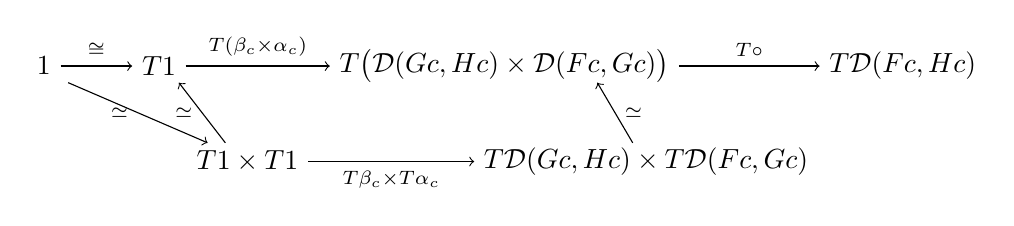
\begin{tikzpicture}[x=1.6em,y=1.5em]
  \node (a1) at (0,2.3) {$1$};
  \node (a2) at (2.6,2.3) {$T1$};
  \node (a3) at (10.4,2.3)
    {$T\bigl(\mathcal{D}(Gc,Hc)\times\mathcal{D}(Fc,Gc)\bigr)$};
  \node (a4) at (19.4,2.3) {$T\mathcal{D}(Fc,Hc)$};
  \draw[->] (a1) -- node[above]{$\scriptstyle\cong$} (a2);
  \draw[->] (a2) -- node[above]{$\scriptstyle T(\beta_{c}\times\alpha_{c})$} (a3);
  \draw[->] (a3) -- node[above]{$\scriptstyle T\circ$} (a4);
  \node (b1) at (4.6,0) {$T1\times T1$};
  \node (b2) at (13.6,0)
    {$T\mathcal{D}(Gc,Hc)\times T\mathcal{D}(Fc,Gc)$};
  \draw[->] (b1) -- node[below]{$\scriptstyle T\beta_{c}\times T\alpha_{c}$} (b2);
  \draw[->] (0.55,1.9) -- node[left,pos=0.5]{$\scriptstyle\simeq$} (3.7,0.45);
  \draw[->] (4.1,0.45) -- node[left]{$\scriptstyle\simeq$} (3.05,1.9);
  \draw[->] (13.3,0.45) -- node[right]{$\scriptstyle\simeq$} (12.5,1.9);
\end{tikzpicture}
\end{center}
该方块由\trIsomorphism{} $T(u\times v)\cong Tu\times Tv$ 的自然性而交换，而
三角形之所以交换，是因为 $1$ 是\trTerminal{}对象，于是所示诸\trIsomorphism{}%
之逆构成一个交换三角形。水平复合之函子性的论证类似。
\end{proof}

\begin{remark}\label{rem:change-of-base-2-functorial}
事实上，「换基」这一程序 $\mathcal{V}\mapsto\mathcal{V}\text{-}\Cat$
\emph{本身}就是一支 2-\trFunctor：从由\trCartesianClosed{}范畴、保持有限积的%
\trFunctor{}与\trNaturalTransformation{}构成的 2-\trCategory，到由 2-范畴、
2-\trFunctor{}与 2-自然变换构成的 2-\trCategory。讨论与证明见
\cite[\S\,4.3]{bib31}。
\end{remark}

作为\cref{rem:change-of-base-2-functorial}之 2-函子性的一个直接推论：

\begin{proposition}\label{prop:change-of-base-2-adjunction}
任何一支介于\trCartesianClosed{}范畴之间、其左伴随保持有限积的\trAdjunction，
都诱导一个换基 2-伴随
\begin{center}
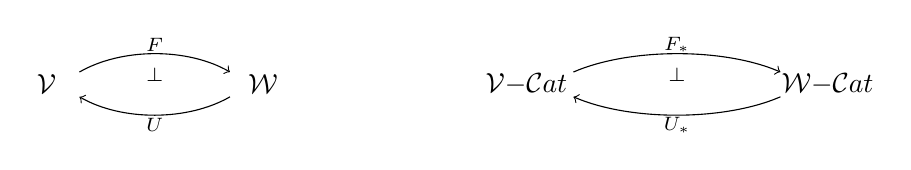
\begin{tikzpicture}[x=1.7em,y=1.4em]
  \node (v) at (0,0) {$\mathcal{V}$};
  \node (w) at (4.6,0) {$\mathcal{W}$};
  \draw[->] (0.7,0.32) .. controls (1.6,0.95) and (3.0,0.95) .. (3.9,0.32);
  \node at (2.3,1.02) {$\scriptstyle F$};
  \node at (2.3,0.25) {$\scriptstyle\bot$};
  \draw[->] (3.9,-0.32) .. controls (3.0,-0.95) and (1.6,-0.95) .. (0.7,-0.32);
  \node at (2.3,-1.05) {$\scriptstyle U$};
  \node at (7.4,0) {$\scriptstyle\rightsquigarrow$};
  \begin{scope}[shift={(10.2,0)}]
    \node (vc) at (0,0) {$\mathcal{V}\text{-}\Cat$};
    \node (wc) at (6.4,0) {$\mathcal{W}\text{-}\Cat$};
    \draw[->] (1.0,0.32) .. controls (2.2,0.95) and (4.2,0.95) .. (5.4,0.32);
    \node at (3.2,1.02) {$\scriptstyle F_{*}$};
    \node at (3.2,0.25) {$\scriptstyle\bot$};
    \draw[->] (5.4,-0.32) .. controls (4.2,-0.95) and (2.2,-0.95) .. (1.0,-0.32);
    \node at (3.2,-1.05) {$\scriptstyle U_{*}$};
  \end{scope}
\end{tikzpicture}
\end{center}
\end{proposition}

\begin{proof}
当然，右伴随总是保持积的，故\trFunctor{}伴随对 $F\dashv U$ 在
\cref{rem:change-of-base-2-functorial}所描述的那个「\trCartesianClosed{}范畴
与保持有限积的\trFunctor」之 2-\trCategory{}中定义一个\trAdjunction。于是，
2-\trFunctor{} $\mathcal{V}\mapsto\mathcal{V}\text{-}\Cat$ 把左侧所示的%
\trAdjunction{}带到右侧所示的\trAdjunction。
\end{proof}

作为一个特例：

\begin{corollary}\label{cor:underlying-free-2-adjunction}
对任何容有\trCoproduct{}的\trCartesianClosed{}范畴 $\mathcal{V}$，取底范畴的
构造与取自由范畴的构造定义一对伴随的 2-\trFunctor
\begin{center}
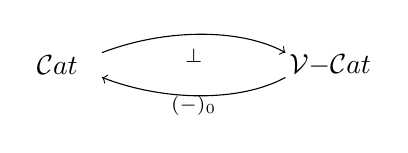
\begin{tikzpicture}[x=1.7em,y=1.4em]
  \node (c) at (0,0) {$\Cat$};
  \node (vc) at (5.8,0) {$\mathcal{V}\text{-}\Cat$};
  \draw[->] (0.95,0.32) .. controls (2.3,0.95) and (3.9,0.95) .. (4.85,0.32);
  \node at (2.9,0.25) {$\scriptstyle\bot$};
  \draw[->] (4.85,-0.32) .. controls (3.9,-0.95) and (2.3,-0.95) .. (0.95,-0.32);
  \node at (2.9,-1.05) {$\scriptstyle(-)_{0}$};
\end{tikzpicture}
\end{center}
\end{corollary}

鉴于\cref{prop:change-of-base-2-adjunction}与随后的诸结果，一支介于%
\trCartesianClosed{}范畴之间、其左伴随保持有限积的\trAdjunction{}提供一个
\textbf{换基伴随}（change-of-base adjunction）。
\cref{prop:change-of-base-2-adjunction}容许沿一支保持有限积的\trAdjunction{}%
的任一伴随作换基，而接下来的一系列结果将揭示：沿右伴随的换基表现要更好一些。

\begin{lemma}\label{lem:finite-product-adjunction-v-enriched}
任何一支由介于\trCartesianClosed{}范畴之间的、保持有限积的诸\trFunctor{}构成
的\trAdjunction
\begin{center}
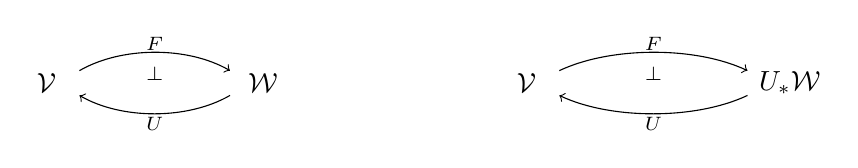
\begin{tikzpicture}[x=1.7em,y=1.4em]
  \node (v) at (0,0) {$\mathcal{V}$};
  \node (w) at (4.6,0) {$\mathcal{W}$};
  \draw[->] (0.7,0.32) .. controls (1.6,0.95) and (3.0,0.95) .. (3.9,0.32);
  \node at (2.3,1.02) {$\scriptstyle F$};
  \node at (2.3,0.25) {$\scriptstyle\bot$};
  \draw[->] (3.9,-0.32) .. controls (3.0,-0.95) and (1.6,-0.95) .. (0.7,-0.32);
  \node at (2.3,-1.05) {$\scriptstyle U$};
  \node at (7.4,0) {$\scriptstyle\rightsquigarrow$};
  \begin{scope}[shift={(10.2,0)}]
    \node (v2) at (0,0) {$\mathcal{V}$};
    \node (uw) at (5.6,0) {$U_{*}\mathcal{W}$};
    \draw[->] (0.7,0.32) .. controls (1.8,0.95) and (3.6,0.95) .. (4.7,0.32);
    \node at (2.7,1.02) {$\scriptstyle F$};
    \node at (2.7,0.25) {$\scriptstyle\bot$};
    \draw[->] (4.7,-0.32) .. controls (3.6,-0.95) and (1.8,-0.95) .. (0.7,-0.32);
    \node at (2.7,-1.05) {$\scriptstyle U$};
  \end{scope}
\end{tikzpicture}
\end{center}
都在诸 $\mathcal{V}$-范畴 $\mathcal{V}$ 与 $U_{*}\mathcal{W}$ 之间定义一个
$\mathcal{V}$-富集\trAdjunction；亦即，存在一个 $\mathcal{V}$-自然%
\trIsomorphism
\[ UW(Fv,w)\cong\mathcal{V}(v,Uw). \]
\end{lemma}

\begin{proof}
$\mathcal{V}$-函子 $U\colon U_{*}\mathcal{W}\to\mathcal{V}$ 的内部作用
$U_{a,b}\colon UW(a,b)\to\mathcal{V}(Ua,Ub)$ 定义为映射
$U\mathrm{ev}\colon UW(a,b)\times Ua\to Ub$ 的转置，后者由把 $U$ 施于
$\mathcal{W}$ 的\trCartesianClosed{}伴随之余单位而得。交换方块
\eqref{eq:composition-transpose-square}提供了这个映射的 $\mathcal{V}$-函子性。

由 $U\colon U_{*}\mathcal{W}\to\mathcal{V}$ 的 $\mathcal{V}$-函子性，映射
\[ UW(Fv,w)\xrightarrow{\ U_{Fv,w}\ }\mathcal{V}(UFv,Uw)
   \xrightarrow{\ -\circ\eta_{v}\ }\mathcal{V}(v,Uw) \]
对一切 $v\in\mathcal{V}$ 都在 $w\in U_{*}\mathcal{W}$ 中是 $\mathcal{V}$-自然
的。由\cref{rem:vleft-adjoint-representability}，为给 $F$ 构造一个相容的
$\mathcal{V}$-富集，只需证明这个映射是 $\mathcal{V}$ 中的一个\trIsomorphism。

我们通过构造一个显式的逆来做到这一点，即
\[ \mathcal{V}(v,Uw)\xrightarrow{\ \eta\ }UF\mathcal{V}(v,Uw)
   \xrightarrow{\ U(F_{v,Uw})\ }UW(Fv,FUw)
   \xrightarrow{\ \varepsilon_{w}\circ-\ }UW(Fv,w) \]
其中中间那个映射定义为：把非富集\trFunctor{} $U$ 施于来自 $\mathcal{W}$-函子
$F\colon F_{*}\mathcal{V}\to\mathcal{W}$ 的作用映射，而该 $\mathcal{W}$-函子
的定义方式与 $\mathcal{V}$-函子 $U\colon U_{*}\mathcal{W}\to\mathcal{V}$ 类似。

这两个映射互逆的证明涉及一对图表追索，其中第一幅表明：右上复合约化到左下复合，
而后者是恒同：
\begin{center}
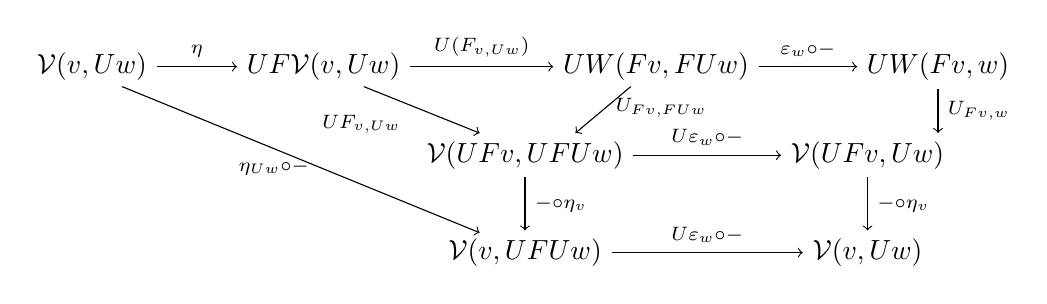
\begin{tikzpicture}[x=1.82em,y=1.6em]
  \node (a) at (0,3.2) {$\mathcal{V}(v,Uw)$};
  \node (b) at (4.6,3.2) {$UF\mathcal{V}(v,Uw)$};
  \node (c) at (11.2,3.2) {$UW(Fv,FUw)$};
  \node (d) at (16.8,3.2) {$UW(Fv,w)$};
  \draw[->] (a) -- node[above]{$\scriptstyle\eta$} (b);
  \draw[->] (b) -- node[above]{$\scriptstyle U(F_{v,Uw})$} (c);
  \draw[->] (c) -- node[above]{$\scriptstyle\varepsilon_{w}\circ-$} (d);
  \node (e) at (8.6,1.2) {$\mathcal{V}(UFv,UFUw)$};
  \node (f) at (15.4,1.2) {$\mathcal{V}(UFv,Uw)$};
  \draw[->] (e) -- node[above]{$\scriptstyle U\varepsilon_{w}\circ-$} (f);
  \draw[->] (10.7,2.75) -- node[right,pos=0.45]{$\scriptstyle U_{Fv,FUw}$} (9.6,1.7);
  \draw[->] (16.8,2.7) -- node[right]{$\scriptstyle U_{Fv,w}$} (16.8,1.7);
  \draw[->] (5.4,2.75) -- node[below left,pos=0.4]{$\scriptstyle UF_{v,Uw}$} (7.7,1.7);
  \node (g) at (15.4,-1.0) {$\mathcal{V}(v,Uw)$};
  \draw[->] (15.4,0.7) -- node[right]{$\scriptstyle-\circ\eta_{v}$} (15.4,-0.5);
  \node (h) at (8.6,-1.0) {$\mathcal{V}(v,UFUw)$};
  \draw[->] (8.6,0.7) -- node[right]{$\scriptstyle-\circ\eta_{v}$} (8.6,-0.5);
  \draw[->] (h) -- node[above]{$\scriptstyle U\varepsilon_{w}\circ-$} (g);
  \draw[->] (0.6,2.75) -- node[left,pos=0.55]{$\scriptstyle\eta_{Uw}\circ-$} (7.7,-0.55);
\end{tikzpicture}
\end{center}
唯一的微妙之处在于梯形区域的交换性，它表达这样一个事实：$\eta\colon\allowbreak\mathrm{id}_{\mathcal{V}}\Rightarrow UF$
是介于\trCartesianClosed{}范畴之间的、保持积的诸\trFunctor{}之间的一个
\emph{闭自然变换}（closed natural transformation）。该区域之所以交换，是因为
其转置后的图表交换：
\begin{center}
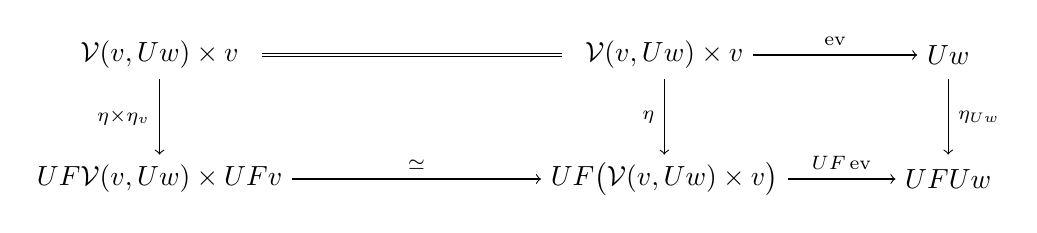
\begin{tikzpicture}[x=1.9em,y=1.6em]
  \node (t1) at (0,1.7) {$\mathcal{V}(v,Uw)\times v$};
  \node (t2) at (9.6,1.7) {$\mathcal{V}(v,Uw)\times v$};
  \node (t3) at (15.0,1.7) {$Uw$};
  \draw[double,double distance=0.6pt] (1.95,1.7) -- (7.65,1.7);
  \draw[->] (t2) -- node[above]{$\scriptstyle\mathrm{ev}$} (t3);
  \node (b1) at (0,-1.1) {$UF\mathcal{V}(v,Uw)\times UFv$};
  \node (b2) at (9.6,-1.1) {$UF\bigl(\mathcal{V}(v,Uw)\times v\bigr)$};
  \node (b3) at (15.0,-1.1) {$UFUw$};
  \draw[->] (b1) -- node[above]{$\scriptstyle\simeq$} (b2);
  \draw[->] (b2) -- node[above]{$\scriptstyle UF\,\mathrm{ev}$} (b3);
  \draw[->] (0,1.15) -- node[left]{$\scriptstyle\eta\times\eta_{v}$} (0,-0.55);
  \draw[->] (9.6,1.15) -- node[left]{$\scriptstyle\eta$} (9.6,-0.55);
  \draw[->] (15.0,1.15) -- node[right]{$\scriptstyle\eta_{Uw}$} (15.0,-0.55);
\end{tikzpicture}
\end{center}
右侧方块由自然性而交换，而左侧方块之所以交换，则是因为介于保持积的诸%
\trFunctor{}之间的任何\trNaturalTransformation{}都自动是一个幺半自然变换
（见\cref{ex:monoidal-functors}）。另一幅图表追索类似。
\end{proof}

\begin{proposition}\label{prop:change-of-base-tensored-cotensored}
给定一支介于\trCartesianClosed{}范畴之间的\trAdjunction
\begin{center}
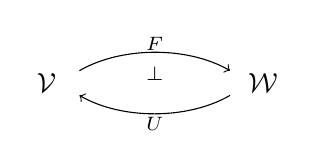
\begin{tikzpicture}[x=1.7em,y=1.4em]
  \node (v) at (0,0) {$\mathcal{V}$};
  \node (w) at (4.6,0) {$\mathcal{W}$};
  \draw[->] (0.7,0.32) .. controls (1.6,0.95) and (3.0,0.95) .. (3.9,0.32);
  \node at (2.3,1.02) {$\scriptstyle F$};
  \node at (2.3,0.25) {$\scriptstyle\bot$};
  \draw[->] (3.9,-0.32) .. controls (3.0,-0.95) and (1.6,-0.95) .. (0.7,-0.32);
  \node at (2.3,-1.05) {$\scriptstyle U$};
\end{tikzpicture}
\end{center}
其左伴随保持有限积。若 $\mathcal{C}$ 作为 $\mathcal{W}$-范畴是余/张量化的，
则 $U_{*}\mathcal{C}$ 作为 $\mathcal{V}$-范畴是余/张量化的，其中 $c\in\mathcal{C}$
经 $v\in\mathcal{V}$ 的余/张量由
\[ v\otimes c\coloneqq Fv\otimes c
   \qquad\text{以及}\qquad
   c^{v}\coloneqq c^{Fv} \]
定义。
\end{proposition}

\begin{proof}
设 $\mathcal{C}$ 作为 $\mathcal{W}$-范畴容有余张量。为验证 $U_{*}\mathcal{C}$
作为 $\mathcal{V}$-范畴容有余张量，我们必须供给一个居于 $\mathcal{V}$ 之中、
在 $x$ 上 $\mathcal{V}$-自然的\trIsomorphism
\[ U\mathcal{C}(x,c^{Fv})\cong\bigl(U\mathcal{C}(x,c)\bigr)^{v} \]
由富集\trYonedaLemma，我们可以从一个在 $u\in\mathcal{V}$ 上 $\mathcal{V}$-自
然的\trIsomorphism
\[ \mathcal{V}\bigl(u,U\mathcal{C}(x,c^{Fv})\bigr)
   \cong\mathcal{V}\bigl(u,\bigl(U\mathcal{C}(x,c)\bigr)^{v}\bigr) \]
中提取出这个\trIsomorphism。为此，把\cref{lem:finite-product-adjunction-v-enriched}
的诸 $\mathcal{V}$-自然\trIsomorphism、源自 $\mathcal{V}$ 与 $\mathcal{W}$%
\footnote{原书此处印作「on $\mathcal{V}$ and on $U_{*}\mathcal{W}$」；按下方
同构链中 $UW\bigl(Fu,\mathcal{C}(x,c)^{Fv}\bigr)\cong UW\bigl(Fu\times Fv,\mathcal{C}(x,c)\bigr)$ 一步系施用 $\mathcal{W}$ 的%
\trCartesianClosed{}结构，而 $U_{*}\mathcal{W}$ 系 $\mathcal{V}$-范畴、本无
笛卡尔封闭结构可言，疑为 $\mathcal{W}$ 之误，此处径改。——译者注}
上\trCartesianClosed{}结构的那些富集自然\trIsomorphism、以及刻画 $\mathcal{C}$
上的余张量并表达 $F$ 保持二元\trProduct{}这一事实的那些\trIsomorphism{}复合%
起来，便有：
\begin{align*}
\mathcal{V}\bigl(u,U\mathcal{C}(x,c^{Fv})\bigr)
  &\cong UW\bigl(Fu,\mathcal{C}(x,c^{Fv})\bigr)
   \cong UW\bigl(Fu,\mathcal{C}(x,c)^{Fv}\bigr)\\
  &\cong UW\bigl(Fu\times Fv,\mathcal{C}(x,c)\bigr)
   \cong UW\bigl(F(u\times v),\mathcal{C}(x,c)\bigr)\\
  &\cong\mathcal{V}\bigl(u\times v,U\mathcal{C}(x,c)\bigr)
   \cong\mathcal{V}\bigl(u,\bigl(U\mathcal{C}(x,c)\bigr)^{v}\bigr).
\end{align*}
\end{proof}

这套换基理论，从富集范畴的复合名词视角看固然很好，但形容词的观点还会生出一层
额外的关切。若保持有限积的\trFunctor{} $T\colon\mathcal{V}\to\mathcal{W}$ 在
自然\trIsomorphism{}的意义下与 $\mathcal{V}$ 和 $\mathcal{W}$ 的底集函子交换，
则由\cref{rem:change-of-base-2-functorial}的 2-函子性，换基 2-函子
$T_{*}\colon\mathcal{V}\text{-}\Cat\to\mathcal{W}\text{-}\Cat$ 也在自然%
\trIsomorphism{}的意义下保持诸底范畴。这特别地发生于如下设定中。

\begin{lemma}\label{lem:change-of-base-underlying-categories}
考虑一支介于\trCartesianClosed{}范畴之间的、保持有限积的\trAdjunction：
\begin{center}
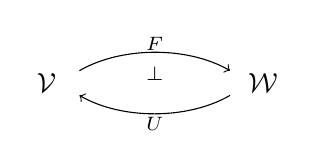
\begin{tikzpicture}[x=1.7em,y=1.4em]
  \node (v) at (0,0) {$\mathcal{V}$};
  \node (w) at (4.6,0) {$\mathcal{W}$};
  \draw[->] (0.7,0.32) .. controls (1.6,0.95) and (3.0,0.95) .. (3.9,0.32);
  \node at (2.3,1.02) {$\scriptstyle F$};
  \node at (2.3,0.25) {$\scriptstyle\bot$};
  \draw[->] (3.9,-0.32) .. controls (3.0,-0.95) and (1.6,-0.95) .. (0.7,-0.32);
  \node at (2.3,-1.05) {$\scriptstyle U$};
\end{tikzpicture}
\end{center}
那么，沿右伴随的换基尊重诸底范畴：
\begin{center}
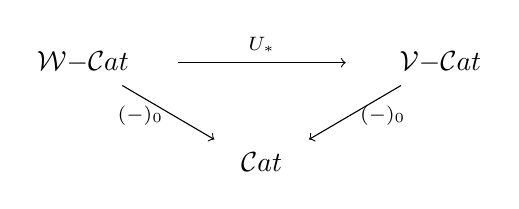
\begin{tikzpicture}[x=1.9em,y=1.5em]
  \node (wc) at (0,1.3) {$\mathcal{W}\text{-}\Cat$};
  \node (vc) at (6.8,1.3) {$\mathcal{V}\text{-}\Cat$};
  \draw[->] (1.8,1.3) -- node[above]{$\scriptstyle U_{*}$} (5.0,1.3);
  \node (cat) at (3.4,-1.1) {$\Cat$};
  \draw[->] (0.75,0.75) -- node[left,pos=0.55]{$\scriptstyle(-)_{0}$} (2.5,-0.55);
  \draw[->] (6.05,0.75) -- node[right,pos=0.55]{$\scriptstyle(-)_{0}$} (4.3,-0.55);
\end{tikzpicture}
\end{center}
\end{lemma}

\begin{proof}
设 $\mathcal{C}$ 是一个 $\mathcal{W}$-范畴。$U_{*}\mathcal{C}$ 的底范畴中从
$x$ 到 $y$ 的 hom-集，同构于 $\mathcal{C}$ 的底范畴中相应的 hom-集
\[ U_{*}\mathcal{C}(x,y)_{0}
   \cong\mathcal{V}\bigl(1,U\mathcal{C}(x,y)\bigr)_{0}
   \cong\mathcal{W}\bigl(F1,\mathcal{C}(x,y)\bigr)_{0}
   \cong\mathcal{W}\bigl(1,\mathcal{C}(x,y)\bigr)_{0}
   \cong\mathcal{C}(x,y)_{0} \]
而且这个\trIsomorphism{}尊重诸底范畴中的复合与单位。于是
$\mathcal{C}_{0}\cong U_{*}\mathcal{C}_{0}$。类似的论证表明：沿 $U$ 的换基
尊重底\trFunctor{}与底\trNaturalTransformation。
\end{proof}

我们以重返第 1 章中的\cref{dig:change-of-base}所预演过的一个例子，来为本章
收尾。

\begin{example}\label{exa:homotopy-nerve-change-of-base}
第 1 章中的\cref{prop:nerve-left-adjoint}的\trAdjunction
\begin{center}
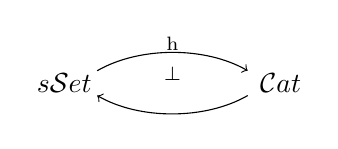
\begin{tikzpicture}[x=1.7em,y=1.4em]
  \node (ss) at (0,0) {$\sSet$};
  \node (ct) at (4.6,0) {$\Cat$};
  \draw[->] (0.7,0.32) .. controls (1.6,0.95) and (3.0,0.95) .. (3.9,0.32);
  \node at (2.3,1.02) {$\scriptstyle\mathrm{h}$};
  \node at (2.3,0.25) {$\scriptstyle\bot$};
  \draw[->] (3.9,-0.32) .. controls (3.0,-0.95) and (1.6,-0.95) .. (0.7,-0.32);
\end{tikzpicture}
\end{center}
之两个伴随都保持有限积。于是，\cref{prop:change-of-base-2-adjunction}诱导一个
由 2-\trFunctor
\begin{center}
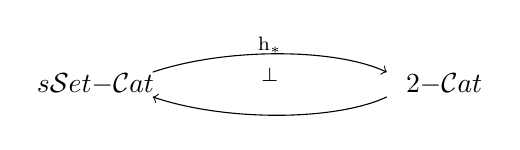
\begin{tikzpicture}[x=1.8em,y=1.4em]
  \node (sc) at (0,0) {$\sSet\text{-}\Cat$};
  \node (tc) at (7.0,0) {$2\text{-}\Cat$};
  \draw[->] (1.15,0.32) .. controls (2.6,0.95) and (4.8,0.95) .. (5.85,0.32);
  \node at (3.5,1.02) {$\scriptstyle\mathrm{h}_{*}$};
  \node at (3.5,0.25) {$\scriptstyle\bot$};
  \draw[->] (5.85,-0.32) .. controls (4.8,-0.95) and (2.6,-0.95) .. (1.15,-0.32);
\end{tikzpicture}
\end{center}
定义的换基伴随，它们在对象上的作用相同，而在 hom 上则分别施用%
\trHomotopyCategory{}函子或\trNerve{}函子。由
\cref{lem:change-of-base-underlying-categories}，右伴随——它从一个
2-\trCategory{}造出一个\trSimpliciallyEnrichedCategory——尊重底范畴：由对象
与 1-\trCell{}构成的底范畴，被等同于由对象与 0-箭头构成的底范畴。在此情形，
\trFunctor{} $\mathrm{h}\colon\sSet\to\Cat$ 与诸底集函子交换，故事实上两个伴
随都保持底范畴，这从直接计算也显而易见。特别地，一个\trInfinityCosmos{}的%
\trHomotopyTwoCategory{}具有相同的底 1-\trCategory。
\end{example}

\subsection*{练习}

\begin{exercise}\label{ex:monoidal-functors}
查阅幺半函子（monoidal functor）与幺半变换（monoidal transformation）的定义
——它们有时被称作\emph{松幺半函子}（lax monoidal functor）与\emph{松幺半变
换}（lax monoidal transformation）——并证明：
\begin{enumerate}[label=(\roman*)]
\item 带有限积的诸\trCategory{}之间的任何保持积的\trFunctor{}都是幺半的；并且
\item 这类\trFunctor{}之间的任何\trNaturalTransformation{}都是一个幺半自然
  变换。
\end{enumerate}
\end{exercise}

\begin{exercise}\label{ex:tensors-cotensors-underlying}
设 $\mathcal{V}$ 是一个\trCartesianClosed{}范畴，并设 $\mathcal{C}$ 是一个张
量化且余张量化的 $\mathcal{V}$-范畴。由
\cref{prop:change-of-base-tensored-cotensored}，底范畴 $\mathcal{C}_{0}$ 作为
一个非富集范畴是张量化且余张量化的。请描述这些张量与余张量。
\end{exercise}

   %
